\documentclass[10pt]{article}
\usepackage{float}
\usepackage{adjustbox}
\usepackage[margin=1.0in]{geometry}
\usepackage{graphicx}
\usepackage{booktabs}
\usepackage{amsmath}
\usepackage{caption}
\usepackage{subcaption}
\usepackage{hyperref}
\usepackage{rotating}
\usepackage{multicol}
\usepackage{tabularx}
\usepackage{xurl}
\def\UrlBreaks{\do\/\do-\do\.\do\_}
\usepackage{url}
\usepackage[utf8]{inputenc}
\usepackage{graphicx}
\usepackage{subcaption}
\usepackage{float}

\title{\textbf{Modelo Probabilístico de Previsão de Resultados de Futebol na Liga Portuguesa}}
\author{Francisca Mateus\\
\texttt{uc2023212096@student.uc.pt} \\ \\
Faculdade de Ciências e Tecnologias da Universidade de Coimbra
\\ \\Licenciatura em Inteligência Artificial e Ciência de Dados\\Inteligência Artificial Probabílistica\\ 
}

\date{}
\graphicspath{{Imagens/}}

\begin{document}

\maketitle

\section{Introdução}

\subsection{Contexto}
O futebol é um domínio caracterizado por uma elevada incerteza, onde o resultado final de um jogo depende de uma multiplicidade de fatores dinâmicos e estocásticos.Tradicionalmente, a previsão de resultados baseava-se na intuição de especialistas, contudo, a crescente disponibilidade de dados granulares permitiu a ascensão da modelagem probabilística. No contexto das apostas desportivas, a capacidade de quantificar a incerteza não é apenas uma vantagem teórica, mas uma necessidade prática, pois modelos que conseguem estimar probabilidades mais precisas do que as oferecidas pelas casas de apostas permitem identificar situações de ``valor'', onde a utilidade esperada de uma decisão supera o risco associado. 
\subsection{Objetivos}
O objetivo central deste trabalho é o desenvolvimento e a implementação de um sistema robusto de previsão probabilística para os resultados (Vitória, Empate, Derrota) de jogos da Liga Portuguesa de Futebol. Para tal, o projeto propõe-se a:
\begin{itemize}
    \item Construir e comparar Redes Bayesianas baseadas tanto em conhecimento especializado como em algoritmos de aprendizagem de estrutura.
    \item Implementar classificadores probabilísticos e avaliar a sua calibração e incerteza através de técnicas como \textit{Conformal Prediction}.
    \item Aplicar a Teoria de Utilidade para transformar previsões probabilísticas em decisões de aposta estratégicas, comparando o desempenho do modelo com as \textit{odds} reais de mercado.
\end{itemize}

\subsection{Dataset e Pré-processamento}
Para este estudo, utilizou-se um conjunto de dados histórico da liga portuguesa contendo informações detalhadas sobre os confrontos, golos e as \textit{odds} iniciais. O dataset original foi sujeito a um processo rigoroso de feature engineering para capturar a dinâmica competitiva das equipas, destacando-se variáveis como:
\begin{itemize}
    \item \textbf{\texttt{ht\_form} e \texttt{at\_form}:} Indicadores de forma recente para as equipas da casa e visitante.
    \item \textbf{\texttt{ht\_attack} e \texttt{at\_attack}:} Métricas que quantificam o poder ofensivo.
    \item \textbf{\texttt{odds\_favorite}:} Variável que sintetiza a expetativa do mercado.
\end{itemize}
O pré-processamento incluiu a limpeza de valores omissos e a discretização de variáveis contínuas, garantindo que os dados estivessem num formato adequado para a aprendizagem de parâmetros.

\section{Redes Bayesianas}
\subsection{Construção da Estrutura}
\subsubsection{Configuração do Ambiente e Preparação de Dados}

O fluxo de trabalho iniciou-se com uma etapa de filtragem onde foram selecionadas as variáveis mais relevantes para a modelação probabilística. Designadamente, consideraram-se a forma recente das equipas (\texttt{ht\_form}, \texttt{at\_form}), o potencial ofensivo (\texttt{ht\_attack}, \texttt{at\_attack}), o histórico de confrontos diretos (\texttt{h2h\_dominance}) e a tendência do mercado (\texttt{odds\_favorite}), variáveis discretizadas. Complementarmente, realizou-se uma análise exploratória inicial, focada na distribuição percentual das classes do resultado final ($H, D, A$), de forma a compreender as tendências base do domínio.
\begin{figure}[H]
    \centering
    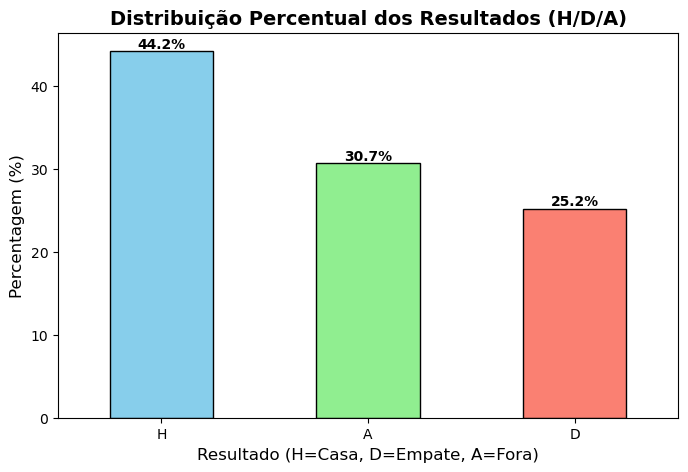
\includegraphics[width=0.7\textwidth]{Dist_resultado.png}
    \caption{Distribuição percentual dos resultados na Liga Portuguesa (H: Casa, D: Empate, A: Fora).}
    \label{fig:dist_resultados}
\end{figure}

\noindent
A análise da distribuição dos resultados, apresentada na Figura \ref{fig:dist_resultados}, revela uma clara predominância de vitórias das equipas visitadas (Home). Esta assimetria estatística é fundamental para a modelação probabilística, uma vez que as probabilidades \textit{a priori} do nosso sistema devem refletir esta tendência natural do domínio antes de considerarmos as métricas específicas de performance de cada equipa.
\subsubsection{Abordagem Baseada em Engenharia de Conhecimento}
A primeira abordagem na modelação da Rede Bayesiana consistiu na técnica de \textit{Knowledge Engineering}, onde a estrutura do Grafo Acíclico Dirigido(DAG) foi definida manualmente. O objetivo foi mapear as relações causais e as dependências lógicas que regem o domínio do futebol profissional, utilizando as variáveis discretizadas do \textit{dataset}.

As ligações definidas no modelo manual podem ser agrupadas em quatro eixos lógicos:

\begin{itemize}
    \item \textbf{Desempenho e Forma:} As variáveis de ataque (\texttt{ht\_attack} e \texttt{at\_attack}) foram ligadas às respetivas variáveis de forma (\texttt{ht\_form} e \texttt{at\_form}). A lógica reside no facto de que uma elevada capacidade ofensiva é o motor principal para a obtenção de pontos e, consequentemente, para a manutenção de uma forma positiva ao longo da época.
    
    \item \textbf{Determinantes das Odds:} Considerou-se que as casas de apostas (\texttt{odds\_favorite}) baseiam as suas avaliações na forma recente das equipas e no histórico de confrontos diretos (\texttt{h2h\_dominance}). Assim, estas três variáveis convergem para o nó das \textit{odds}, refletindo como o mercado processa a informação histórica.
    
    \item \textbf{Influências Diretas no Resultado:} O desfecho do jogo (\texttt{result}) é influenciado diretamente pelo potencial ofensivo das equipas e pela dominância histórica entre elas. Estas ligações capturam a componente técnica e psicológica que define quem tem maior probabilidade de vencer o confronto.
    
    \item \textbf{Informação Latente do Mercado:} A ligação da variável \texttt{odds\_favorite} ao \texttt{result} justifica-se pelo facto de as \textit{odds} funcionarem como um agregador de informação latente que não está explicitamente no \textit{dataset} (como lesões de última hora, castigos de jogadores-chave ou condições meteorológicas), mas que tem impacto direto no resultado final.
\end{itemize}

\begin{figure}[H]
    \centering
    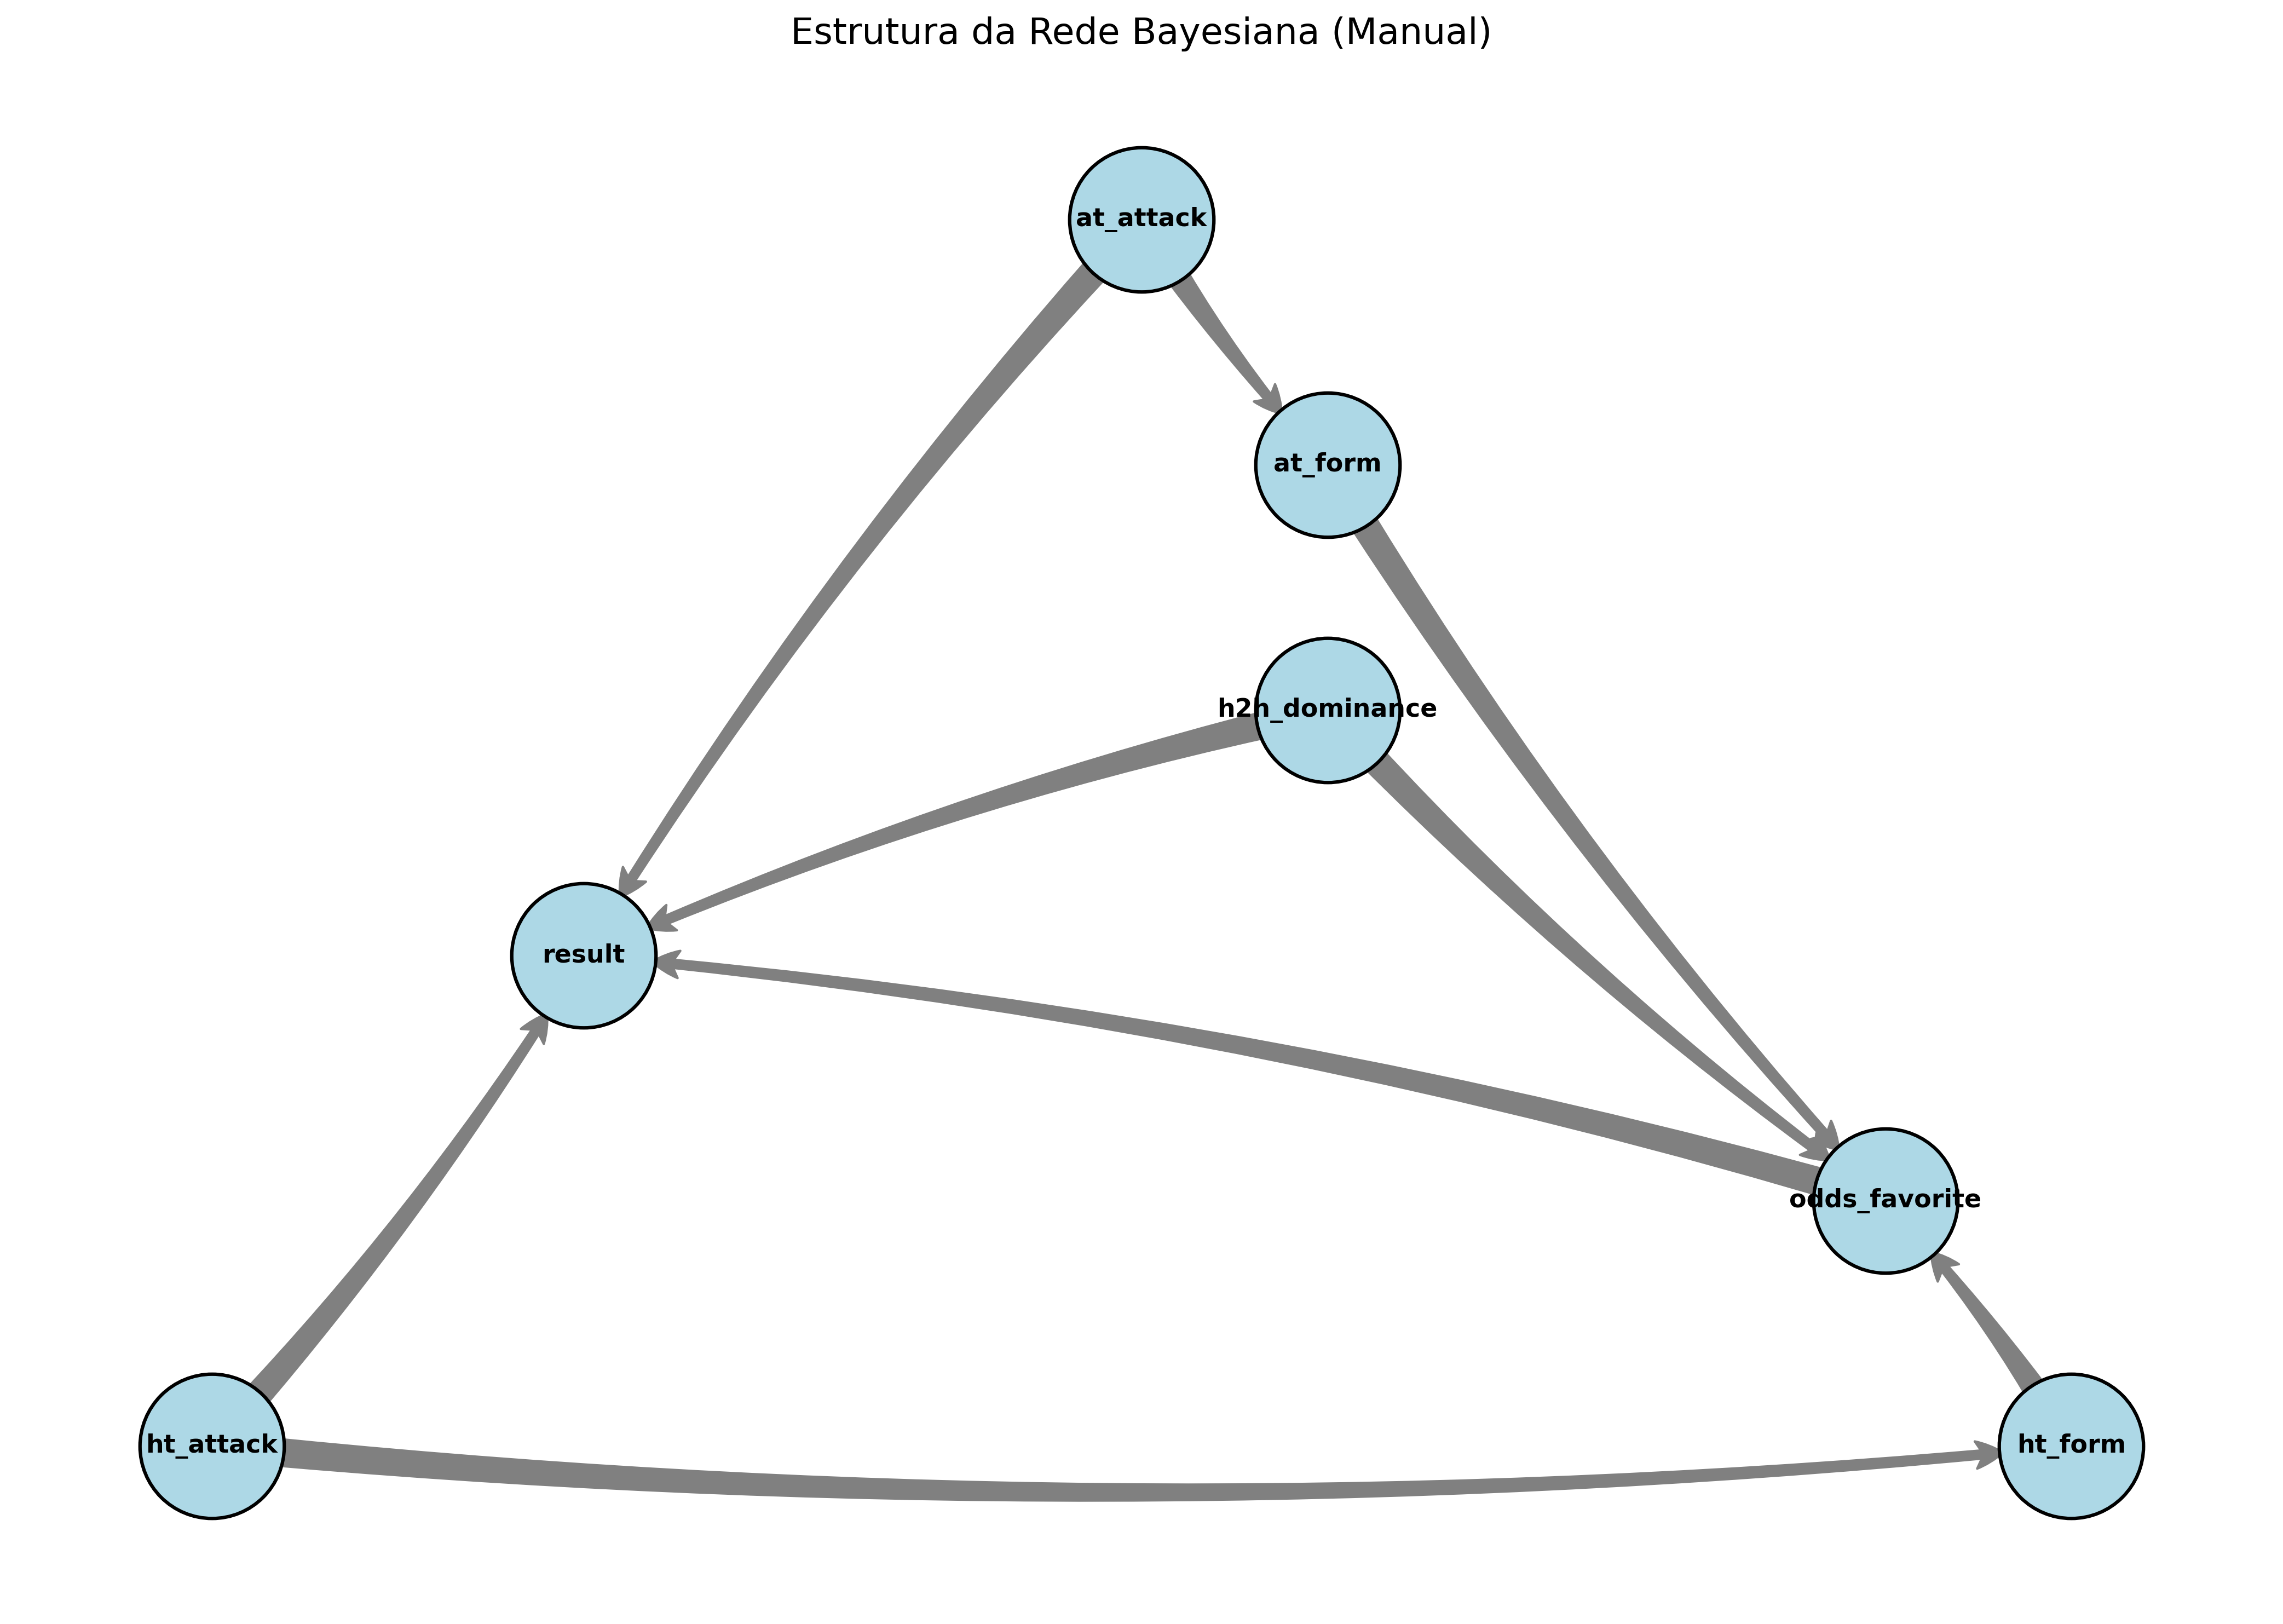
\includegraphics[width=0.8\textwidth]{dag_manual.png} 
    \caption{Estrutura da Rede Bayesiana definida via Engenharia de Conhecimento.}
    \label{fig:dag_manual}
\end{figure}

\subsection{Aprendizagem Automática de Estrutura}

Para complementar a abordagem baseada em conhecimento, implementou-se uma estratégia de aprendizagem de estrutura, puramente baseada nos dados. O objetivo desta etapa é identificar correlações e dependências estatísticas que podem não ser óbvias através da análise intuitiva do domínio.

\subsubsection{Algoritmo Hill Climb Search e Métrica BIC}
Utilizou-se o algoritmo \textbf{Hill Climb Search}, uma técnica de procura heurística que explora o espaço de todos os Grafos Acíclicos Dirigidos possíveis. O algoritmo opera realizando operações locais e avaliando cada mudança através de uma função de pontuação.

A função de pontuação escolhida foi o \textbf{Bayesian Information Criterion (BIC)}. A métrica BIC é particularmente adequada para este problema pois equilibra dois fatores fundamentais:
\begin{enumerate}
    \item \textbf{Verosimilhança (Likelihood):} Quão bem a estrutura explica os dados observados.
    \item \textbf{Penalização de Complexidade:} O BIC penaliza estruturas com excesso de parâmetros, prevenindo o \textit{overfitting} e favorecendo modelos mais simples que generalizam melhor para novos jogos.
\end{enumerate}

\subsubsection{Análise da Estrutura Aprendida}

\begin{figure}[H]
    \centering
    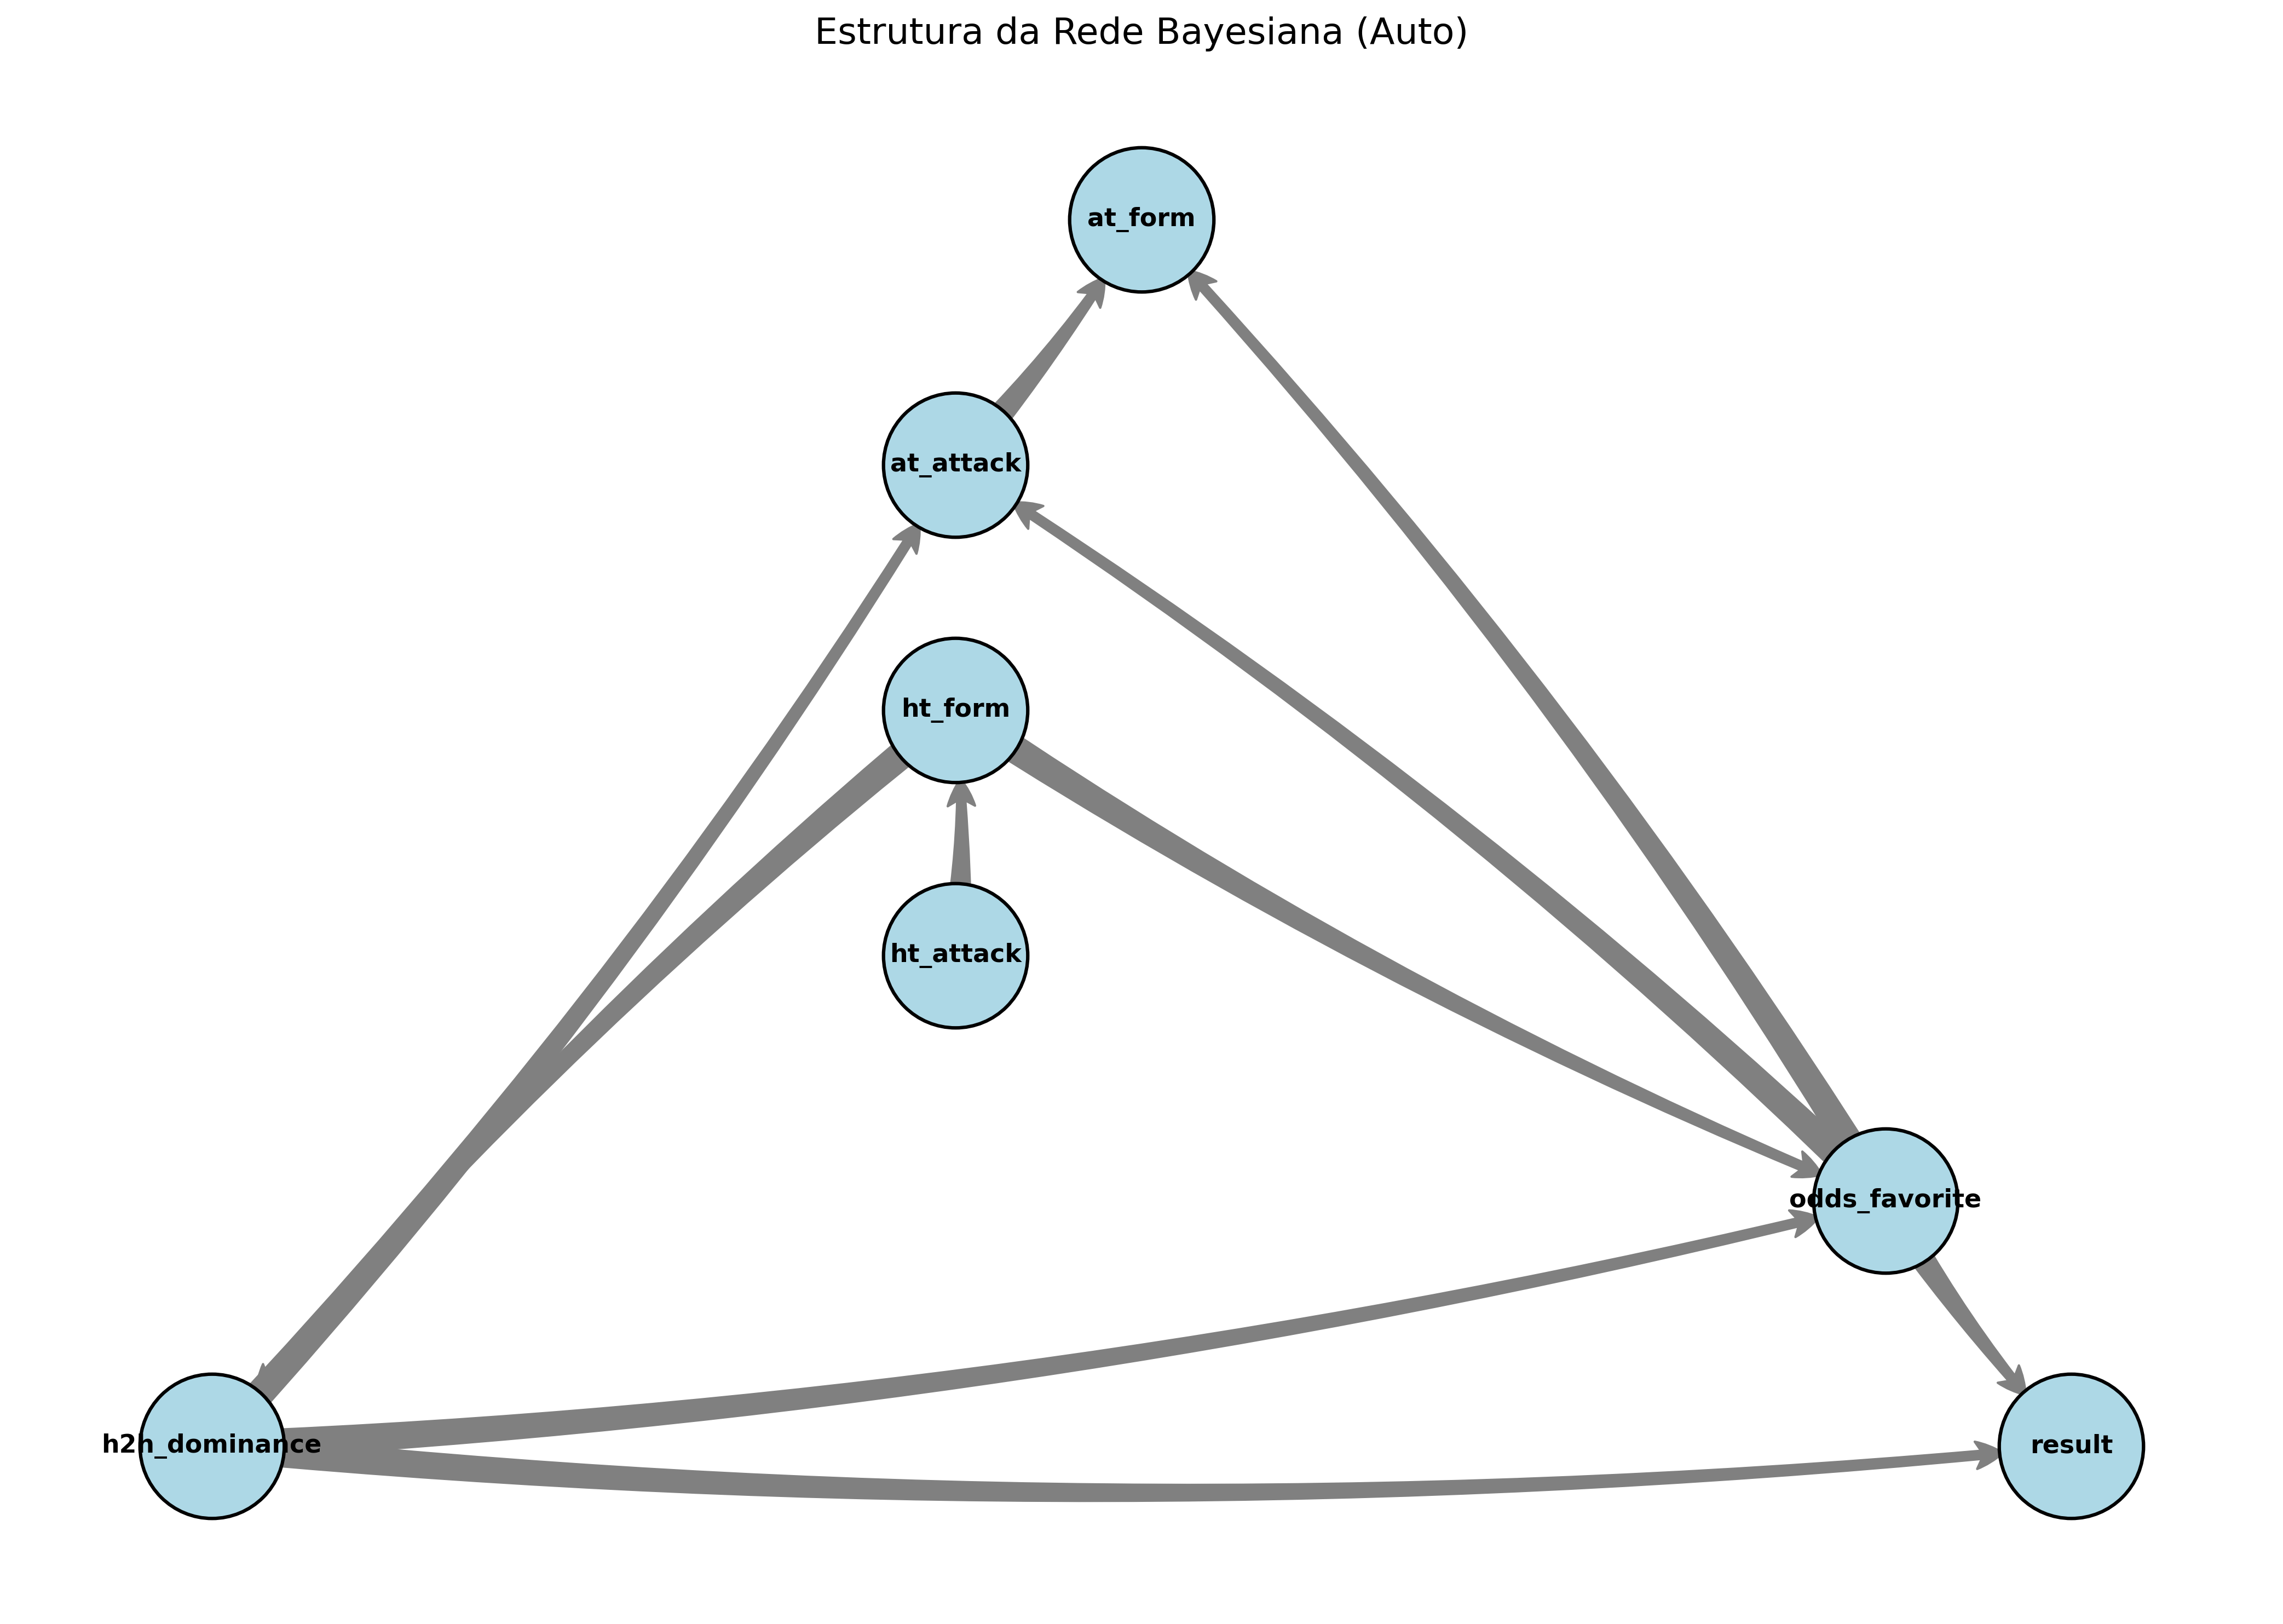
\includegraphics[width=0.8\textwidth]{dag_auto.png}
    \caption{Estrutura da Rede Bayesiana aprendida automaticamente através do algoritmo Hill Climb Search com score BIC.}
    \label{fig:dag_auto}
\end{figure}

\subsubsection{Análise da Estrutura Aprendida e Comparação com o Modelo Manual}

A análise comparativa entre o modelo manual e o modelo automático revela as nuances entre a causalidade teórica e a correlação estatística. 

\paragraph{Validação Estatística de Pressupostos Manuais}
Observa-se que diversas arestas fundamentais foram mantidas na estrutura automática, o que valida estatisticamente as nossas hipóteses iniciais. As ligações \texttt{ht\_attack $\rightarrow$ ht\_form} e \texttt{at\_attack $\rightarrow$ at\_form} permanecem inalteradas, confirmando que a capacidade ofensiva é o motor primário da forma recente. Da mesma forma, as arestas que convergem para o desfecho final, nomeadamente \texttt{odds\_favorite $\rightarrow$ result} e \texttt{h2h\_dominance $\rightarrow$ result}, foram validadas pelo algoritmo. Isto demonstra que, independentemente da complexidade da rede, o histórico de confrontos e as probabilidades de mercado são os preditores mais robustos da performance real na Liga Portuguesa.

\paragraph{Divergências entre Causalidade e Correlação Estatística}
Contudo, o modelo automático introduziu arestas que, embora façam sentido estatístico para minimizar o \textit{score} BIC, parecem desafiar a lógica empírica ou a causalidade temporal:
\begin{itemize}
    \item \textbf{Inversão Causal (\texttt{ht\_form $\rightarrow$ h2h\_dominance}):} Enquanto que manualmente assumimos que o histórico (\textit{h2h}) é um dado fixo, o algoritmo sugere que a forma atual ``explica'' o histórico. No plano estatístico, isto acontece porque equipas que estão em boa forma hoje tendem a ser equipas historicamente dominantes, criando uma dependência mútua que o algoritmo resolve com esta direção de aresta.
    \item \textbf{O Nó das Odds como Hub Informativo:} O algoritmo ligou \texttt{odds\_favorite} diretamente a \texttt{at\_attack} e \texttt{at\_form}. Empiricamente, uma \textit{odd} não causa o ataque de uma equipa, contudo, estatisticamente, a \textit{odd} é um agregador de informação tão eficiente que ela se torna um excelente preditor de todas as outras variáveis de performance. O algoritmo prefere esta estrutura porque ela reduz a incerteza global da rede, utilizando a \textit{odd} como uma variável ``resumo'' do estado das equipas.
\end{itemize}

\paragraph{Conclusão da Comparação}
Em suma, enquanto o modelo manual representa um mapa de \textbf{causalidade}, o modelo automático representa um mapa de \textbf{dependências estatísticas}. O facto de o algoritmo ter mantido as ligações core ao \texttt{result} reforça a confiança no sistema, enquanto as novas ligações em torno das \textit{odds} confirmam que o mercado de apostas captura variáveis latentes que o nosso modelo manual tentava isolar individualmente.

\subsection{Análise de Independências Condicionais (D-Separação)}

A estrutura de uma Rede Bayesiana codifica um conjunto de afirmações de independência condicional. Para validar se estas propriedades se mantêm e compreender como a informação se propaga no modelo, utilizou-se o critério da \textbf{d-separação}.

\subsubsection{Independências Locais e Globais}

\paragraph{Modelo Manual:} 
A análise das independências locais no modelo manual revela um padrão importante para o nó \texttt{result}:
\begin{equation*}
    (result \perp at\_form, ht\_form \mid at\_attack, h2h\_dominance, ht\_attack, odds\_favorite)
\end{equation*}
Isto indica que, uma vez conhecidos os pais diretos do resultado (ataque de ambas as equipas, histórico e as \textit{odds}), a informação sobre a forma recente (\texttt{form}) torna-se redundante. Ou seja, a forma influencia o resultado apenas através do seu impacto no ataque e nas \textit{odds}; se estes já estiverem quantificados, a forma não adiciona novo poder preditivo.

\paragraph{Modelo Automático:}
No modelo aprendido via \textit{Hill Climb}, o algoritmo identificou independências globais que otimizam o \textit{score} BIC. Um exemplo relevante é $(at\_attack \perp result \mid h2h\_dominance, odds\_favorite)$, o que sugere que, estatisticamente, as \textit{odds} e o histórico já capturam tanta informação que o ataque da equipa visitante deixa de ser uma variável independente necessária para explicar o desfecho.

\subsubsection{Testes Práticos de D-Separação}

Para validar a implementação, realizaram-se testes em estruturas fundamentais do grafo:

\paragraph{Estrutura em V (Colisor) e o efeito "Explaining Away"}
Analisou-se o caminho entre \texttt{ht\_attack} e \texttt{at\_attack}, que convergem no nó \texttt{result} (\texttt{ht\_attack $\rightarrow$ result $\leftarrow$ at\_attack}).
\begin{itemize}
    \item \textbf{Sem observações:} As variáveis são \textbf{d-separadas}. O facto de uma equipa ter um bom ataque não nos diz nada sobre o ataque da outra equipa antes do jogo começar.
    \item \textbf{Observando \texttt{result}:} As variáveis tornam-se \textbf{dependentes}. Se soubermos que a equipa da casa perdeu, mas sabemos que teve um ataque excelente, isso ``explica'' (ou aumenta a probabilidade) de a equipa de fora ter tido um desempenho ainda superior. Este fenómeno é conhecido como \textit{explaining away}.
\end{itemize}

\paragraph{Estrutura em Cascata (Chain)}
Analisou-se o fluxo informativo no caminho \texttt{ht\_attack $\rightarrow$ ht\_form $\rightarrow$ odds\_favorite}.
\begin{itemize}
    \item \textbf{Sem observações:} O caminho está \textbf{ativo}. O potencial de ataque influencia a forma, que por sua vez influencia as \textit{odds}. Existe uma dependência indireta.
    \item \textbf{Observando \texttt{ht\_form}:} O caminho fica \textbf{bloqueado} (d-separado). Ao conhecermos a forma atual da equipa, o conhecimento sobre o seu potencial de ataque teórico deixa de influenciar a nossa estimativa das \textit{odds}, pois a forma já é o resultado concreto desse ataque.
\end{itemize}

\paragraph{Estrutura em Fork e as Odds como Hub:}
No modelo automático, analisou-se o caminho \texttt{at\_attack $\leftarrow$ odds\_favorite $\rightarrow$ result}, onde as \textit{odds} assumem o papel de causa comum.
\begin{itemize}
    \item \textbf{Sem observações:} O caminho está \textbf{ativo}. Existe uma dependência estatística entre a força do ataque visitante e o resultado, mediada pela perceção do mercado.
    \item \textbf{Observando \texttt{odds\_favorite}:} O caminho fica \textbf{bloqueado} (d-separado). Ao conhecermos a cotação do mercado, a informação sobre o ataque do visitante torna-se redundante para prever o resultado. Isto valida a hipótese de que, nesta rede, as \textit{odds} funcionam como um "hub informativo" que absorve as métricas técnicas.
\end{itemize}

\paragraph{Estrutura em Cascata e Atalhos Estatísticos:}
Avaliou-se a cadeia de dependência \texttt{ht\_attack $\rightarrow$ ht\_form $\rightarrow$ h2h\_dominance}, que reflete uma inversão causal identificada pelo algoritmo.
\begin{itemize}
    \item \textbf{Sem observações:} O caminho está \textbf{ativo}. O potencial de ataque influencia a forma, que por sua vez é usada pelo algoritmo para explicar a dominância histórica.
    \item \textbf{Observando \texttt{ht\_form}:} O caminho fica \textbf{bloqueado}. A forma atual atua como um separador: uma vez conhecido o momento atual da equipa, a ligação entre o seu potencial ofensivo teórico e o histórico de confrontos é interrompida.
\end{itemize}

Este comportamento confirma que as redes implementadas respeitam os axiomas de grafos probabilísticos e que a inferência será realizada sobre caminhos de dependência válidos.

\subsection{Aprendizagem de Parâmetros: MLE vs. Estimação Bayesiana}

Após a definição da estrutura da Rede Bayesiana Manual, a etapa seguinte consistiu em aprender as Tabelas de Probabilidade Condicional (CPTs). Para este efeito, compararam-se duas abordagens distintas: a \textit{Maximum Likelihood Estimation} (MLE) e a \textit{Bayesian Estimation} (utilizando o \textit{prior} BDeu).

A escolha do modelo manual para esta análise deve-se à sua elevada interpretabilidade causal, facilitando a validação das probabilidades aprendidas face ao conhecimento empírico do domínio.

\subsubsection{Comparação Metodológica}

\paragraph{Maximum Likelihood Estimation (MLE):} 
Este método calcula as probabilidades baseando-se estritamente na frequência relativa dos dados. Como observado nos resultados, para a variável \texttt{ht\_form}, quando o \texttt{ht\_attack} é \textit{weak}, a probabilidade de forma \textit{excellent} é de exatamente $0.0000$. Embora reflita fielmente o histórico, esta abordagem sofre do problema da probabilidade nula: se um evento nunca ocorreu no passado, o modelo assume que é impossível, o que pode bloquear processos de inferência futuros.

\paragraph{Estimação Bayesiana (BDeu):}
Para mitigar a rigidez do MLE, aplicou-se a Estimação Bayesiana com um \textit{prior} uniforme equivalente (BDeu). Observando a mesma relação (\texttt{ht\_attack} \textit{weak} $\rightarrow$ \texttt{ht\_form} \textit{excellent}), o valor foi suavizado para $0.000440$. Este processo de \textit{smoothing} introduz ``pseudo-contagens'', garantindo que nenhuma combinação de eventos seja estritamente impossível, conferindo maior robustez ao modelo perante dados esparsos.

\subsubsection{Análise das CPTs e Influência dos Dados}

As tabelas aprendidas revelam como o \textit{dataset} da Liga Portuguesa molda o comportamento do modelo:

\begin{itemize}
    \item \textbf{Impacto do Ataque na Forma:} As CPTs demonstram uma correlação robusta. Por exemplo, uma equipa com \texttt{ht\_attack} \textit{strong} tem uma probabilidade de $49.8\%$ de apresentar forma \textit{excellent}. Inversamente, um ataque \textit{weak} resulta em forma \textit{poor} em $50.4\%$ dos casos.
    \item \textbf{Configuração das Odds:} A variável \texttt{odds\_favorite} atua como um agregador. Quando a equipa da casa é historicamente dominante e está em forma \textit{excellent}, a probabilidade de as \textit{odds} a apontarem como favorita é de $99.7\%$.
    \item \textbf{Determinismo do Resultado:} No nó \texttt{result}, observa-se que em cenários de total favoritismo (Ataque Forte + Histórico Favorável + \textit{Odds} em \textit{Home}), a probabilidade de vitória da casa ($H$) atinge os $82.7\%$. Contudo, o modelo preserva uma margem de incerteza para o empate ($D$) e derrota ($A$), refletindo a imprevisibilidade inerente ao desporto.
\end{itemize}

\paragraph{Conclusão da Aprendizagem}
Embora os valores centrais de ambas as abordagens sejam muito próximos para categorias com muitos dados , a \textbf{Estimação Bayesiana} revelou-se superior para a operacionalização do modelo, ao evitar o determinismo excessivo do MLE em casos raros.

\subsection{Realização de Inferências Probabilísticas}

A grande vantagem de uma Rede Bayesiana sobre classificadores tradicionais é a sua capacidade de realizar inferências em qualquer direção do grafo. Nesta secção, demonstramos a utilização do modelo para responder a cinco questões críticas, utilizando o algoritmo de eliminação de variáveis para calcular as distribuições \textit{a posteriori}.

\subsubsection{Cenários de Previsão e Diagnóstico}

\paragraph{1. Previsão em Cenário de Superioridade:}
Questionou-se o modelo sobre a probabilidade de resultado dado que a equipa da casa apresenta forma \textit{excellent}, ataque \textit{strong} e um histórico \textit{home\_dominant}.
\begin{itemize}
    \item \textbf{Resultado:} $P(H) = 78.5\%$, $P(D) = 14.3\%$, $P(A) = 7.2\%$.
    \item \textbf{Análise:} O modelo demonstra uma elevada confiança na vitória da casa sob estas condições, alinhando-se com a lógica desportiva onde a combinação de forma e superioridade técnica é determinante.
\end{itemize}

\paragraph{2. Inferência Diagnóstica (Causa dado o Efeito):}
Analisou-se um cenário onde a equipa da casa estava em má forma (\textit{poor}) mas conseguiu vencer o jogo ($H$). Qual seria o estado provável da equipa visitante?
\begin{itemize}
    \item \textbf{Resultado:} $P(at\_form \in \{poor, below\ avg\}) \approx 53\%$.
    \item \textbf{Análise:} Perante uma vitória inesperada de uma equipa em má forma, o modelo infere que existe uma probabilidade superior a 50\% de a equipa adversária também estar a atravessar um momento negativo, o que "ajuda a explicar" o desfecho observado.
\end{itemize}

\paragraph{3. Comportamento do Mercado face ao Equilíbrio:}
Num cenário de equilíbrio absoluto (ataques \textit{average} e histórico \textit{balanced}), para onde pendem as \textit{odds}?
\begin{itemize}
    \item \textbf{Resultado:} $P(odds\_favorite = home) = 69.02\%$.
    \item \textbf{Análise:} Mesmo perante o equilíbrio técnico, as casas de apostas mantêm um forte favoritismo para o visitado. Isto reflete o peso estatístico do "fator casa" na Liga Portuguesa, que o modelo aprendeu a incorporar nas suas previsões.
\end{itemize}

\subsubsection{Inter-causalidade e Conflito de Indicadores}

\paragraph{4. Atualização de Perceção por Resultado:}
Avaliou-se a perceção do ataque visitante dado um ataque da casa \textit{strong}, antes e depois de saber que o jogo empatou ($D$).
\begin{itemize}
    \item \textbf{Sem saber o resultado:} $P(at\_attack = above\ avg) = 19.27\%$.
    \item \textbf{Sabendo o Empate (D):} $P(at\_attack = above\ avg) = 24.90\%$.
    \item \textbf{Análise:} O conhecimento do empate força o modelo a "ajustar" a sua perceção sobre a equipa de fora. Se a equipa da casa era forte e o jogo empatou, a probabilidade de a equipa visitante também ter um ataque acima da média sobe quase 6\%, demonstrando o raciocínio inter-causal da rede.
\end{itemize}

\paragraph{5. Conflito entre Mercado e Histórico:}
Se as \textit{odds} favorecem a equipa de fora (\textit{away}), qual a probabilidade de o histórico ser dominado pela equipa da casa?
\begin{itemize}
    \item \textbf{Resultado:} $P(h2h\_dominance = home\_dominant) = 1.39\%$.
    \item \textbf{Análise:} O modelo identifica um conflito extremo. Se o mercado ignora o fator casa para dar favoritismo ao visitante, a probabilidade de existir uma dominância histórica da casa torna-se quase nula. Isto indica que o modelo considera as \textit{odds} como um indicador muito mais atualizado do que o histórico de longo prazo.
\end{itemize}

\section{Classificação Probabilística e Incerteza}

Nesta fase, o objetivo é transitar de um modelo baseado em grafos para classificadores probabilísticos que operam em espaços contínuos. O foco incide na capacidade de prever o desfecho ($H, D, A$) e, simultaneamente, quantificar a confiança do modelo nessas previsões.

\subsection{Preparação e Pré-processamento de Dados}

Antes da fase de modelação, os dados foram submetidos a um pipeline de preparação para garantir a validade estatística dos resultados.

\subsubsection{Limpeza e Seleção de Atributos}
Para evitar o fenómeno de \textit{Data Leakage}, foram removidas variáveis que não estariam disponíveis no momento da previsão ou que codificam diretamente o resultado, designadamente os golos marcados (\texttt{hg}, \texttt{ag}) e identificadores temporais ou de equipa (\texttt{date}, \texttt{ht}, \texttt{at}). 

Após esta limpeza, procedeu-se à separação das características (\textit{features}) em dois grupos:
\begin{itemize}
    \item \textbf{Variáveis Contínuas (18):} Incluem métricas de performance agregada (\texttt{form\_points}, \texttt{goals\_scored}) e as \textit{odds} de mercado, que representam o consenso probabilístico externo.
    \item \textbf{Variáveis Discretas (7):} Categorias resultantes da discretização prévia, como o nível de ataque e dominância histórica.
\end{itemize}
Para os modelos de classificação nesta secção, optou-se por utilizar o conjunto de variáveis contínuas, por preservarem maior granularidade de informação.

\subsubsection{Divisão do Dataset (Train-Calibration-Test)}
Ao contrário de uma divisão binária convencional, os dados foram repartidos em três conjuntos distintos, uma etapa essencial para a implementação futura de \textit{Conformal Prediction}:
\begin{enumerate}
    \item \textbf{Treino (60\%):} Utilizado para a aprendizagem dos parâmetros do modelo.
    \item \textbf{Calibração (20\%):} Reservado exclusivamente para ajustar as probabilidades e definir os \textit{scores} de incerteza sem enviesar o treino.
    \item \textbf{Teste (20\%):} Utilizado para a avaliação final e reporte das métricas de desempenho.
\end{enumerate}

\subsubsection{Normalização e Escalonamento}
Dado que as variáveis apresentam amplitudes muito distintas, aplicou-se a técnica de \textbf{Standardization (Z-score normalization)}. 

É crucial notar que o transformador (\texttt{StandardScaler}) foi ajustado (\textit{fit}) apenas com os dados de treino. A média ($\mu$) e o desvio padrão ($\sigma$) resultantes foram depois aplicados aos conjuntos de calibração e teste. Este procedimento garante que não existe contaminação de informação, assegurando que o modelo é avaliado como se estivesse perante dados genuinamente novos.

\subsection{Treino e Avaliação de Classificadores}
Foram testadas diversas arquiteturas para estabelecer uma \textit{baseline} de desempenho, utilizando parâmetros padrão discutidos em ambiente letivo. Os resultados comparativos encontram-se na Tabela \ref{tab:comparacao_modelos}.

\begin{table}[H]
\centering
\begin{tabular}{lccc}
\hline
\textbf{Modelo} & \textbf{Exatidão} & \textbf{Log Loss} \\ \hline
Logistic Regression & \textbf{0.5336} & \textbf{0.9546}\\
Gradient Boosting & 0.5318 & 0.9763  \\
Random Forest & 0.5192 & 0.9814 \\
SVM (RBF) & 0.5246 & 0.9950 \\
Naive Bayes & 0.4655 & 2.1232 \\
Neural Network (MLP) & 0.4593 & 2.0266\\ \hline
\end{tabular}
\caption{Desempenho comparativo entre os modelos.}
\label{tab:comparacao_modelos}
\end{table}

\paragraph{Análise do Desempenho Comparativo}
A análise comparativa do desempenho dos classificadores revela que a \textbf{Regressão Logística} e o \textbf{Gradient Boosting} são os modelos mais robustos, apresentando as maiores exatidões (aproximadamente 53\%) e os menores valores de \textit{Log Loss} (0.9546 e 0.9763, respetivamente). Estes resultados sugerem que modelos lineares e de \textit{ensemble} conseguem capturar de forma mais eficaz os padrões estatísticos da Liga Portuguesa, mantendo uma incerteza controlada. 

Em contraste, o \textbf{Naive Bayes} apresenta o desempenho mais crítico em termos de probabilidade: embora a sua exatidão não seja a mais baixa, o seu elevado \textit{Log Loss} (2.1232) indica uma calibração deficiente, onde o modelo atribui níveis de confiança excessivamente altos a previsões que acabam por se revelar incorretas. A proximidade dos resultados de exatidão entre os três primeiros modelos indica que o limite preditivo para este \textit{dataset} ronda os 53\%, refletindo a elevada imprevisibilidade inerente ao desfecho de jogos de futebol.


\begin{figure*}[htbp]
    \centering
    % Subfigura 1: Distribuição para Resultado A (Away)
    \begin{subfigure}[b]{0.32\textwidth}
        \centering
        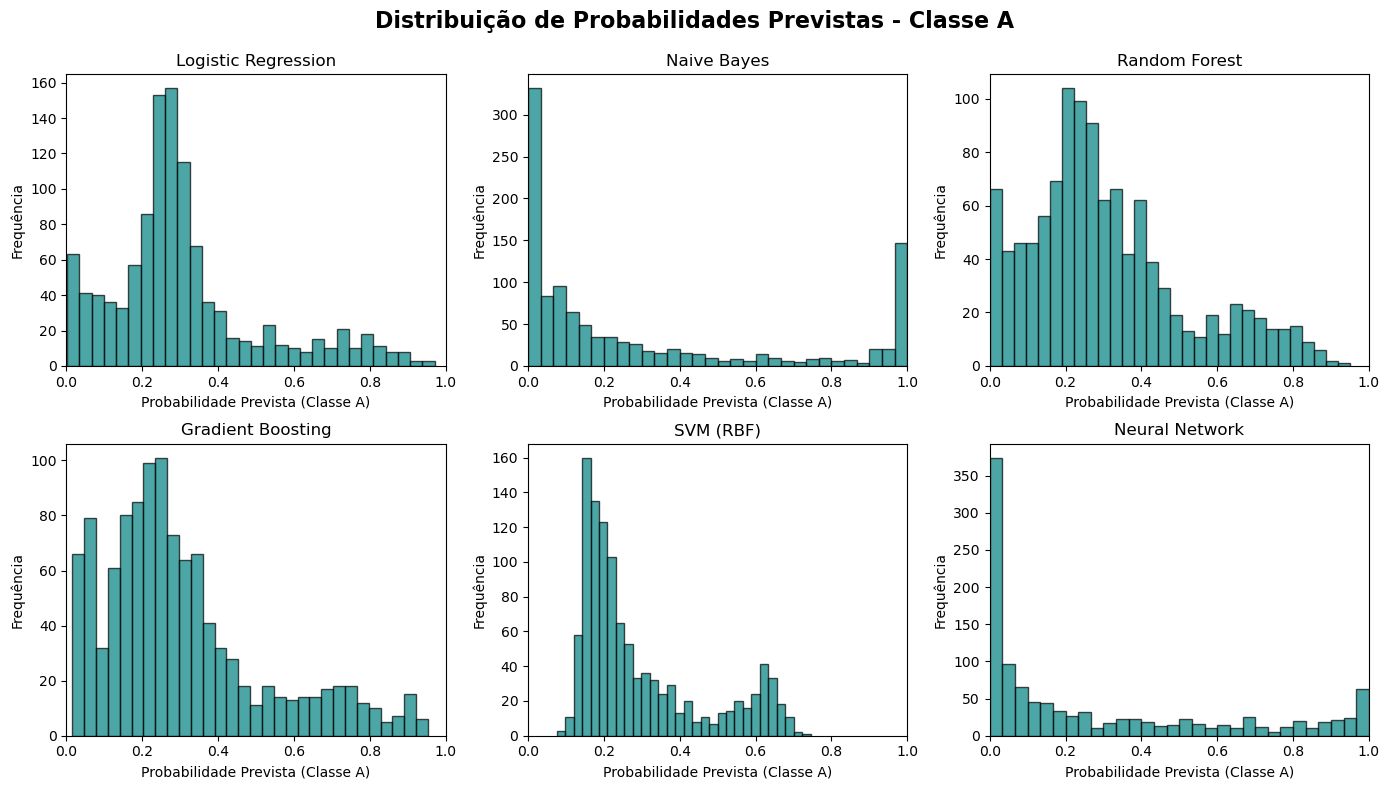
\includegraphics[width=\textwidth]{dist_a.png} % Substituir pelo ficheiro correspondente a 'A'
        \caption{Distribuição de Prob. - Vitória Fora (A)}
        \label{fig:dist_A}
    \end{subfigure}
    \hfill
    % Subfigura 2: Distribuição para Resultado D (Draw)
    \begin{subfigure}[b]{0.32\textwidth}
        \centering
        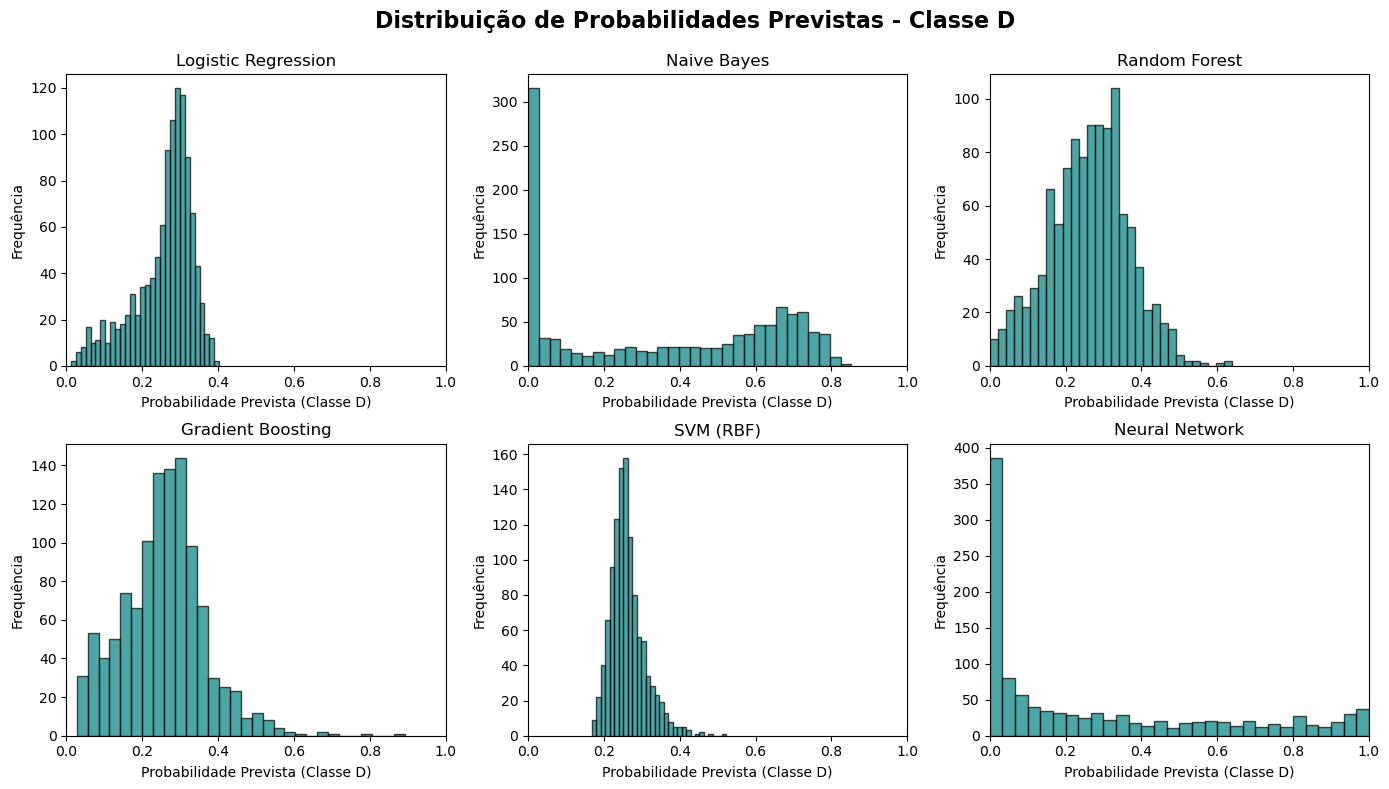
\includegraphics[width=\textwidth]{dist_d.png} % Substituir pelo ficheiro correspondente a 'D'
        \caption{Distribuição de Prob. - Empate (D)}
        \label{fig:dist_D}
    \end{subfigure}
    \hfill
    % Subfigura 3: Distribuição para Resultado H (Home)
    \begin{subfigure}[b]{0.32\textwidth}
        \centering
        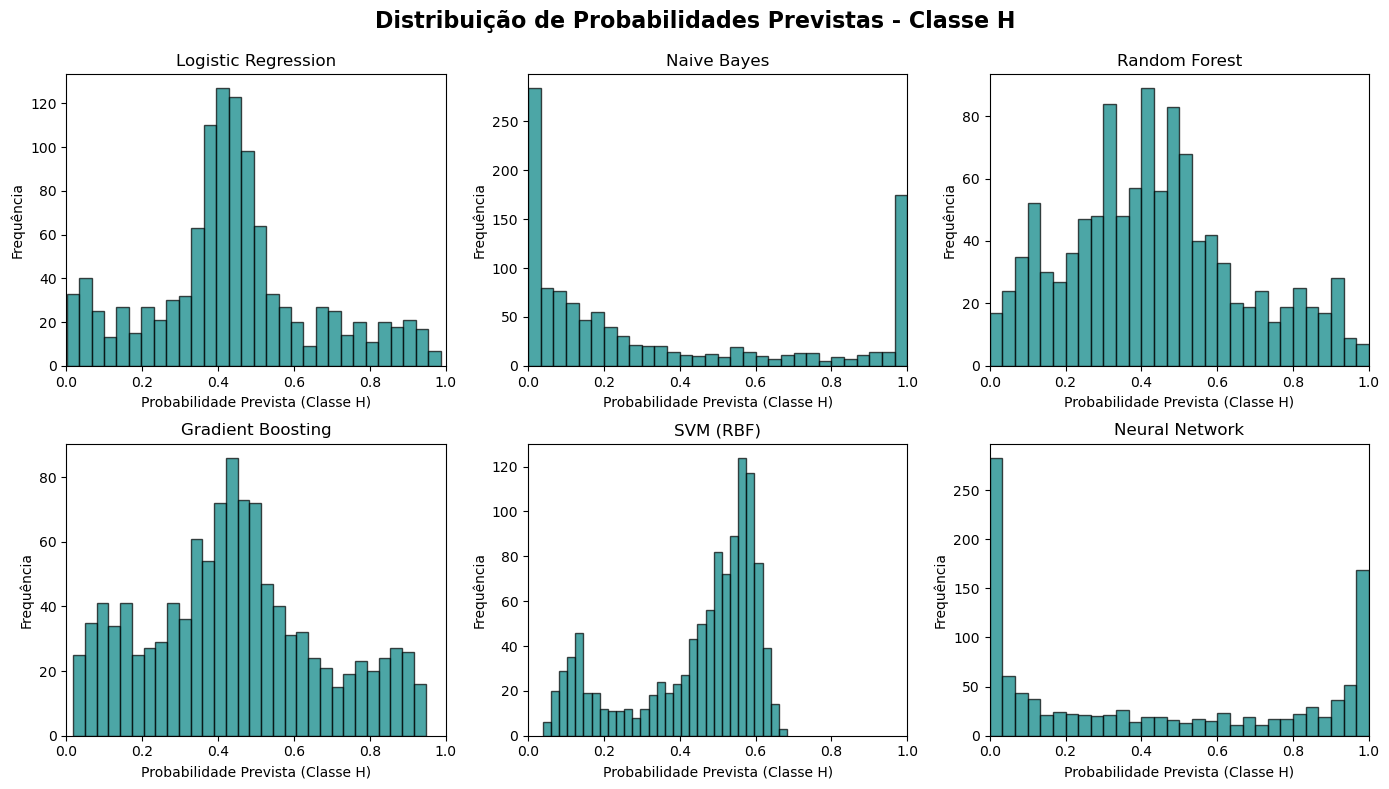
\includegraphics[width=\textwidth]{dist_h.png} % Substituir pelo ficheiro correspondente a 'H'
        \caption{Distribuição de Prob. - Vitória Casa (H)}
        \label{fig:dist_H}
    \end{subfigure}
    
    \caption{Comparação da densidade de probabilidade atribuída pelos diversos classificadores para cada desfecho possível. Cada gráfico sobrepõe o comportamento dos modelos testados para um resultado específico.}
    \label{fig:distribuicoes_probabilidade_comparadas}
\end{figure*}

\paragraph{Análise das Distribuições de Probabilidade por Classe}
A Figura \ref{fig:distribuicoes_probabilidade_comparadas} oferece uma visão detalhada sobre a "certeza" de cada classificador para os três desfechos do jogo. Ao comparar as distribuições, emergem padrões distintos:

\begin{itemize}
    \item \textbf{Vitória em Casa (H):} Na Figura \ref{fig:dist_H}, observa-se que a maioria dos modelos (especialmente a Regressão Logística e SVM) apresenta uma cauda mais longa para a direita. Isto indica que os modelos encontram frequentemente evidência suficiente para atribuir probabilidades elevadas (acima de 60\%) à vitória do visitado, confirmando o peso do fator casa como o preditor mais decisivo no \textit{dataset}.
    
    \item \textbf{Empate (D):} A Figura \ref{fig:dist_D} revela o maior desafio da modelação. A maioria dos classificadores concentra as suas previsões em valores baixos (entre 20\% e 30\%), raramente arriscando uma probabilidade elevada para o empate. O \textbf{Naive Bayes} destaca-se aqui por apresentar uma distribuição mais "achatada" e espalhada, o que explica o seu \textit{recall} superior nesta classe: ele é o único modelo que atribui densidade de probabilidade significativa a cenários de empate onde outros modelos são conservadores.

    \item \textbf{Vitória Fora (A):} Na Figura \ref{fig:dist_A}, as distribuições tendem a ser bimodais ou concentradas em valores intermédios. É visível que os modelos de \textit{ensemble} (Random Forest e Gradient Boosting) são mais cautelosos, evitando atribuir probabilidades extremas de vitória ao visitante, a menos que os indicadores de ataque (\texttt{at\_attack}) sejam excecionalmente superiores aos da casa.
\end{itemize}


\subsection{Quantificação de Incerteza via Conformal Prediction}

Para ultrapassar as limitações das probabilidades pontuais, aplicou-se o \textit{framework} de \textbf{Conformal Prediction} utilizando a biblioteca \texttt{crepes}. O objetivo é gerar conjuntos de previsão (\textit{prediction sets}) que garantam, com um nível de confiança $1-\alpha$, que o resultado real está contido no conjunto.

\subsubsection{Metodologia e Calibração}
Utilizou-se o método \textit{Inductive Conformal Prediction}, tirando partido do conjunto de calibração (20\% dos dados) que não foi visto durante o treino. Para cada modelo, calculou-se o \textit{non-conformity score} baseado na probabilidade da classe correta. Fixou-se um nível de significância $\alpha = 0.1$, visando uma cobertura alvo de 90\%.

\subsubsection{Análise de Resultados e Cobertura}
Os resultados da aplicação aos diversos classificadores estão sintetizados na Tabela \ref{tab:conformal_results}.

\begin{table}[H]
\centering
\begin{tabular}{lccc}
\hline
\textbf{Modelo} & \textbf{Coverage} & \textbf{Target} & \textbf{Mean Set Size} \\ \hline
Logistic Regression & 89.35\% & 90\% & 2.212 \\
\textbf{Naive Bayes} & \textbf{89.17\%} & \textbf{90\%} & \textbf{2.263} \\
Random Forest & 89.44\% & 90\% & 2.328 \\
Gradient Boosting & 88.81\% & 90\% & 2.242 \\
SVM (RBF) & 89.44\% & 90\% & 2.374 \\
Neural Network & 87.56\% & 90\% & 2.383 \\ \hline
\end{tabular}
\caption{Resultados de Conformal Prediction para um nível de confiança de 90\%.}
\label{tab:conformal_results}
\end{table}

\paragraph{Avaliação do Naive Bayes:}
O classificador \textbf{Naive Bayes} obteve uma cobertura de \textbf{89.17\%}, demonstrando uma excelente aderência ao alvo teórico de 90\%. Este resultado é particularmente relevante dado que, apesar de ser um modelo "sobre-confiante" nas suas probabilidades brutas, o processo de conformalização conseguiu corrigir esse viés, forçando a inclusão de mais classes no conjunto de previsão para manter a validade estatística.

\paragraph{Eficiência e Tamanho dos Conjuntos:}
A métrica \textit{Mean Set Size} (tamanho médio do conjunto) revela a "eficiência" do modelo. 
\begin{itemize}
    \item O Naive Bayes apresentou um tamanho médio de \textbf{2.263}. Isto significa que, para garantir 90\% de acerto, o modelo precisa de sugerir, em média, mais de dois desfechos possíveis (ex: $\{H, D\}$ ou $\{D, A\}$).
    \item Comparativamente, a \textbf{Regressão Logística} foi a mais eficiente (2.212), enquanto a \textbf{Rede Neuronal} foi a menos precisa na sua incerteza (2.383), gerando conjuntos mais amplos e, portanto, menos informativos para um apostador.
\end{itemize}

\paragraph{Interpretação Prática:}
O facto de todos os modelos apresentarem um tamanho de conjunto superior a 2.0 indica que o futebol português, sob a ótica destes atributos, contém uma incerteza intrínseca elevada. Raramente o modelo consegue garantir 90\% de confiança com apenas um desfecho, validando a necessidade de abordagens que considerem múltiplos cenários para uma gestão de risco eficaz.

\subsection{Avaliação de Calibração: Reliability Diagrams e Métricas de Erro}

A calibração é a propriedade que garante que, se um modelo prevê uma probabilidade de 70\% para um evento, este deve ocorrer aproximadamente 70\% das vezes. Para avaliar esta componente nos nossos classificadores, utilizámos métricas de erro probabilístico e diagramas de fiabilidade (\textit{Reliability Diagrams}).

\subsubsection{Análise das Métricas: Brier Score e Log Loss}
Os resultados obtidos antes de qualquer processo de calibração explícita encontram-se detalhados na Tabela \ref{tab:metrics_calibration}.

\begin{table}[H]
\centering
\begin{tabular}{lccc}
\hline
\textbf{Classificador} & \textbf{ROC AUC} & \textbf{Brier Score} & \textbf{Log Loss} \\ \hline
Logistic Regression & \textbf{0.6867} & \textbf{0.5632} & \textbf{0.9546} \\
Gradient Boosting & 0.6786 & 0.5785 & 0.9763 \\
Random Forest & 0.6711 & 0.5787 & 0.9814 \\
SVM (RBF) & 0.6390 & 0.5912 & 0.9950 \\
Neural Network & 0.6201 & 0.7742 & 1.6418 \\
Naive Bayes & 0.6762 & 0.7473 & 2.1232 \\ \hline
\end{tabular}
\caption{Métricas de desempenho probabilístico e calibração (sem ajuste).}
\label{tab:metrics_calibration}
\end{table}

O \textbf{Brier Score} indica que a Regressão Logística é o modelo com previsões mais próximas da realidade (0.5632). Por outro lado, o elevado \textbf{Log Loss} do Naive Bayes (2.1232) e da Rede Neuronal (1.6418) confirma que estes modelos penalizam severamente o sistema por atribuírem probabilidades muito elevadas a resultados que acabam por não se verificar.

\subsubsection{Reliability Diagrams por Classe (A, D, H)}
A análise visual das curvas de fiabilidade (Figura \ref{fig:reliability_plots}) permite identificar o comportamento de cada modelo face aos desfechos específicos:

\begin{itemize}
    \item \textbf{Vitória Fora (A) e Casa (H):} Nestas classes, a maioria dos modelos (especialmente Regressão Logística e Gradient Boosting) segue a diagonal de calibração perfeita de forma aceitável. Contudo, o \textbf{Naive Bayes } situa-se sistematicamente abaixo da diagonal em probabilidades altas, o que denuncia um estado de \textbf{sobre-confiança}: o modelo acredita que o favorito ganhará com mais certeza do que a estatística real permite.
    \item \textbf{Empate (D):} Esta é a classe com pior calibração global. Observa-se que quase todos os modelos apresentam curvas "achatadas" ou com declives erráticos. Isto demonstra a dificuldade extrema em calibrar probabilidades para o empate, onde os modelos tendem a subestimar a ocorrência do evento quando a probabilidade prevista é intermédia.
    \item \textbf{Rede Neuronal:} Apresenta um comportamento oscilatório e instável em todas as classes, sugerindo que a sua arquitetura atual falha em produzir estimativas de probabilidade suaves e consistentes.
\end{itemize}

\begin{figure}[H]
    \centering
    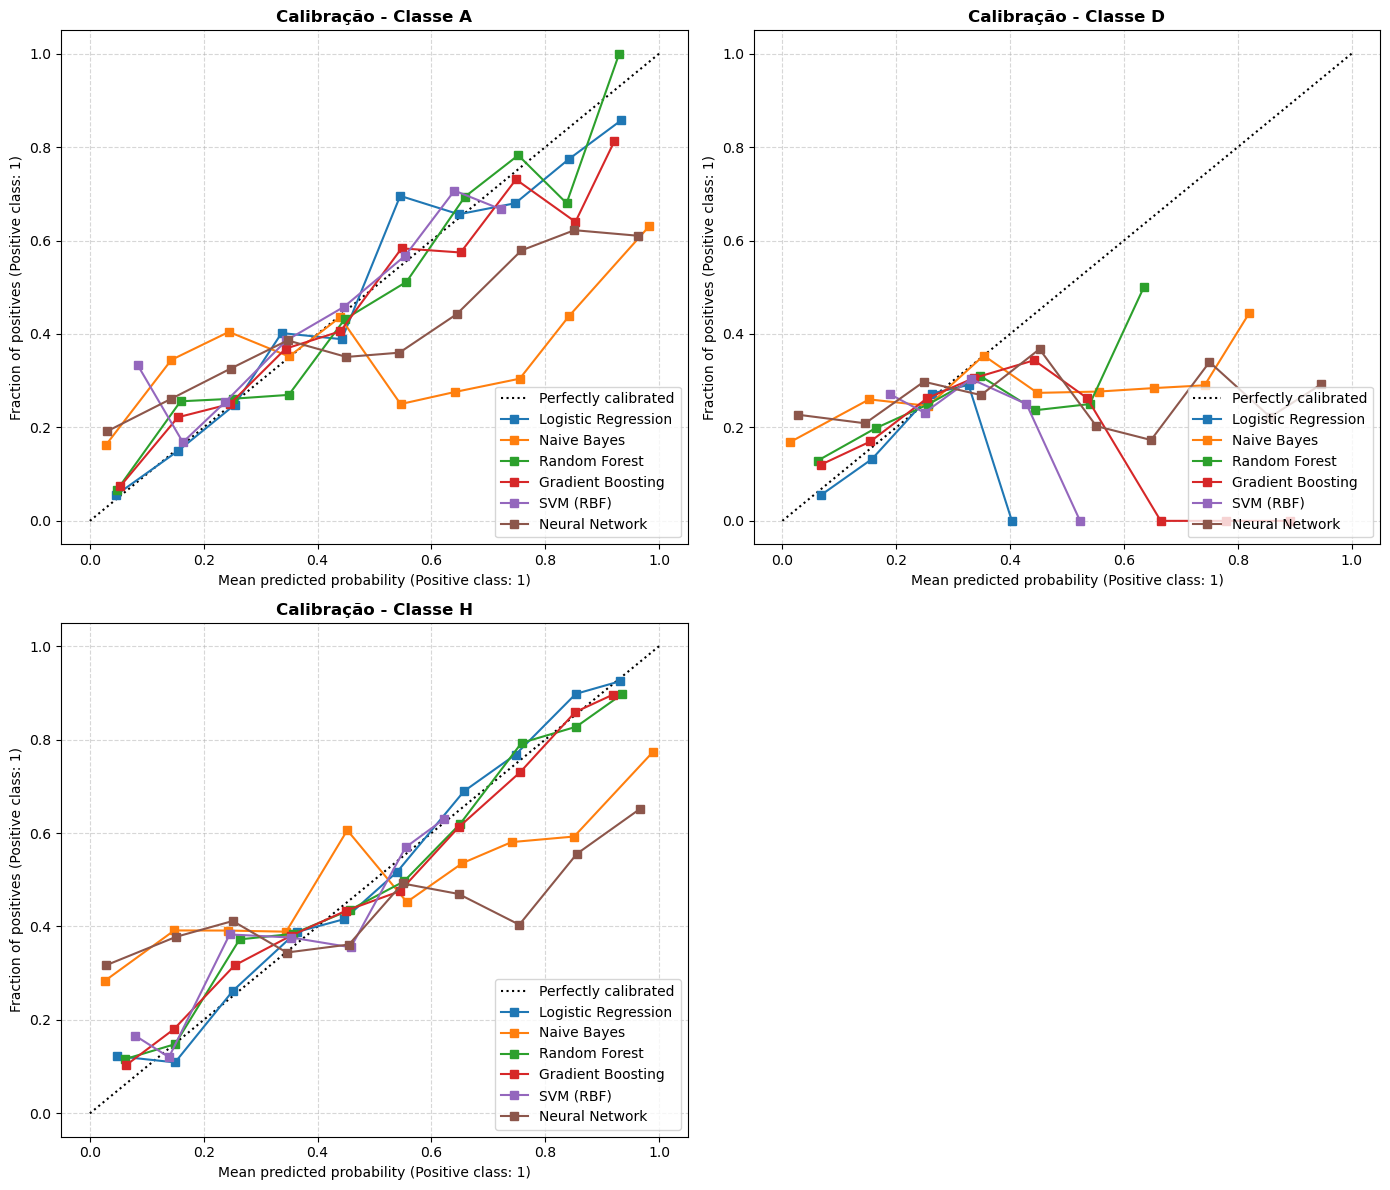
\includegraphics[width=0.95\textwidth]{sem_cal_reliable_diag.png} 
    \caption{Reliability Diagrams comparativos para as classes Vitória Fora (A), Empate (D) e Vitória Casa (H).}
    \label{fig:reliability_plots}
\end{figure}

\paragraph{Conclusão da Calibração:}
A Regressão Logística revela-se o modelo mais equilibrado. O Naive Bayes, apesar de ter um bom poder de discriminação (ROC AUC de 0.6762), requer obrigatoriamente um método de calibração posterior (como \textit{Isotonic Regression}) para que as suas probabilidades possam ser usadas de forma segura na tomada de decisão baseada em utilidade.

\subsubsection{Análise do Impacto dos Métodos de Calibração}

Nesta secção, analisa-se a eficácia das técnicas de calibração \textit{Sigmoid} (Platt Scaling) e \textit{Isotonic Regression} na correção das probabilidades estimadas pelos modelos. Embora a exatidão global tenda a manter-se estável, as métricas probabilísticas revelam transformações profundas na fiabilidade do sistema.

\paragraph{Recuperação de Modelos Sobre-confiantes}
Os benefícios mais expressivos da calibração são observados nos modelos que apresentavam as piores métricas iniciais:
\begin{itemize}
    \item \textbf{Naive Bayes:} Este modelo sofria de uma calibração deficiente (\textit{Log Loss} de 2.1232 e ECE de 0.3082). A aplicação da \textbf{Calibração Isotonic} reduziu o \textit{Log Loss} para \textbf{0.9711} e o ECE para uns impressionantes \textbf{0.0268}. Visualmente, as curvas que anteriormente se afastavam da diagonal de referência passam a segui-la quase perfeitamente em todas as classes (A, D, H).
    \item \textbf{Neural Network:} Semelhante ao Naive Bayes, a rede neuronal reduziu o seu ECE de 0.3356 para \textbf{0.0213} com o método Isotonic. Esta correção é vital, pois transforma um modelo "impreciso na sua confiança" num preditor robusto para análise de risco.
\end{itemize}

\paragraph{Estabilidade em Modelos Lineares e de Ensemble}
Para modelos que já apresentavam uma boa calibração nativa, como a \textbf{Logistic Regression} e o \textbf{Gradient Boosting}, o impacto foi marginal ou, nalguns casos, ligeiramente negativo para o \textit{Log Loss}:
\begin{itemize}
    \item Na \textbf{Logistic Regression}, a configuração sem calibração já apresentava o menor ECE global (0.0240). O método Isotonic degradou ligeiramente o \textit{Log Loss} (de 0.9546 para 1.0210), sugerindo que a complexidade do ajuste não-paramétrico pode introduzir \textit{overfitting} quando o modelo base já é linearmente calibrado.
    \item No \textbf{Gradient Boosting}, o método \textit{Sigmoid} revelou-se superior ao Isotonic, reduzindo o \textit{Log Loss} para 0.9686 e melhorando a consistência das probabilidades.
\end{itemize}

\paragraph{Comparação Isotonic vs. Sigmoid}
De uma forma geral, a \textbf{Isotonic Regression} demonstrou ser a técnica mais poderosa para corrigir desvios sistemáticos não-lineares, especialmente nas classes de difícil previsão como o \textbf{Empate (D)}. Contudo, requer um conjunto de calibração suficientemente grande para evitar o aspeto "em escada" nas previsões. A calibração \textit{Sigmoid} mostrou-se mais conservadora e adequada para modelos onde o erro de calibração segue uma distribuição logística simples.

\begin{figure}[H]
    \centering
    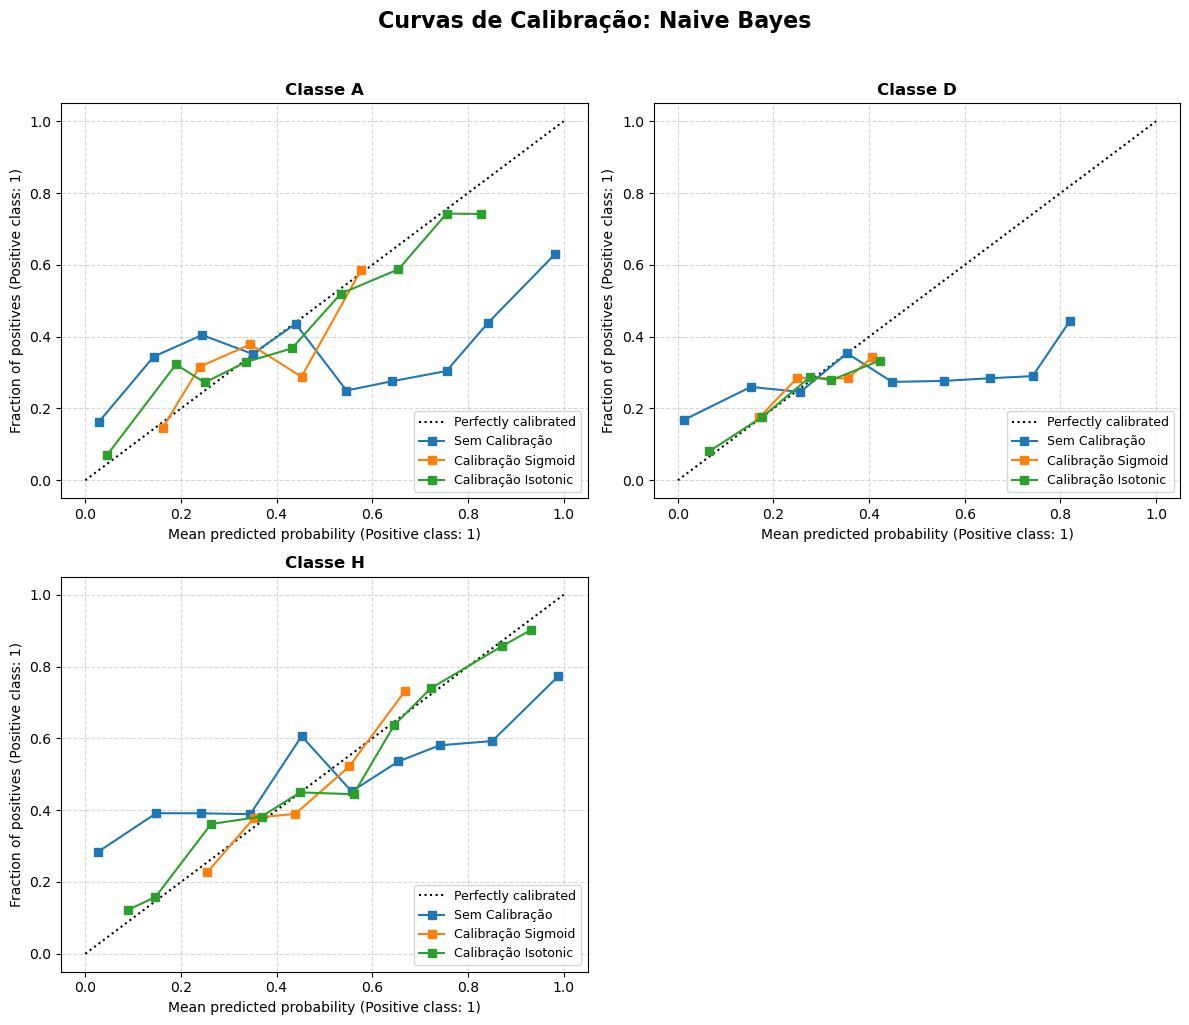
\includegraphics[width=0.45\textwidth]{nb.png}
    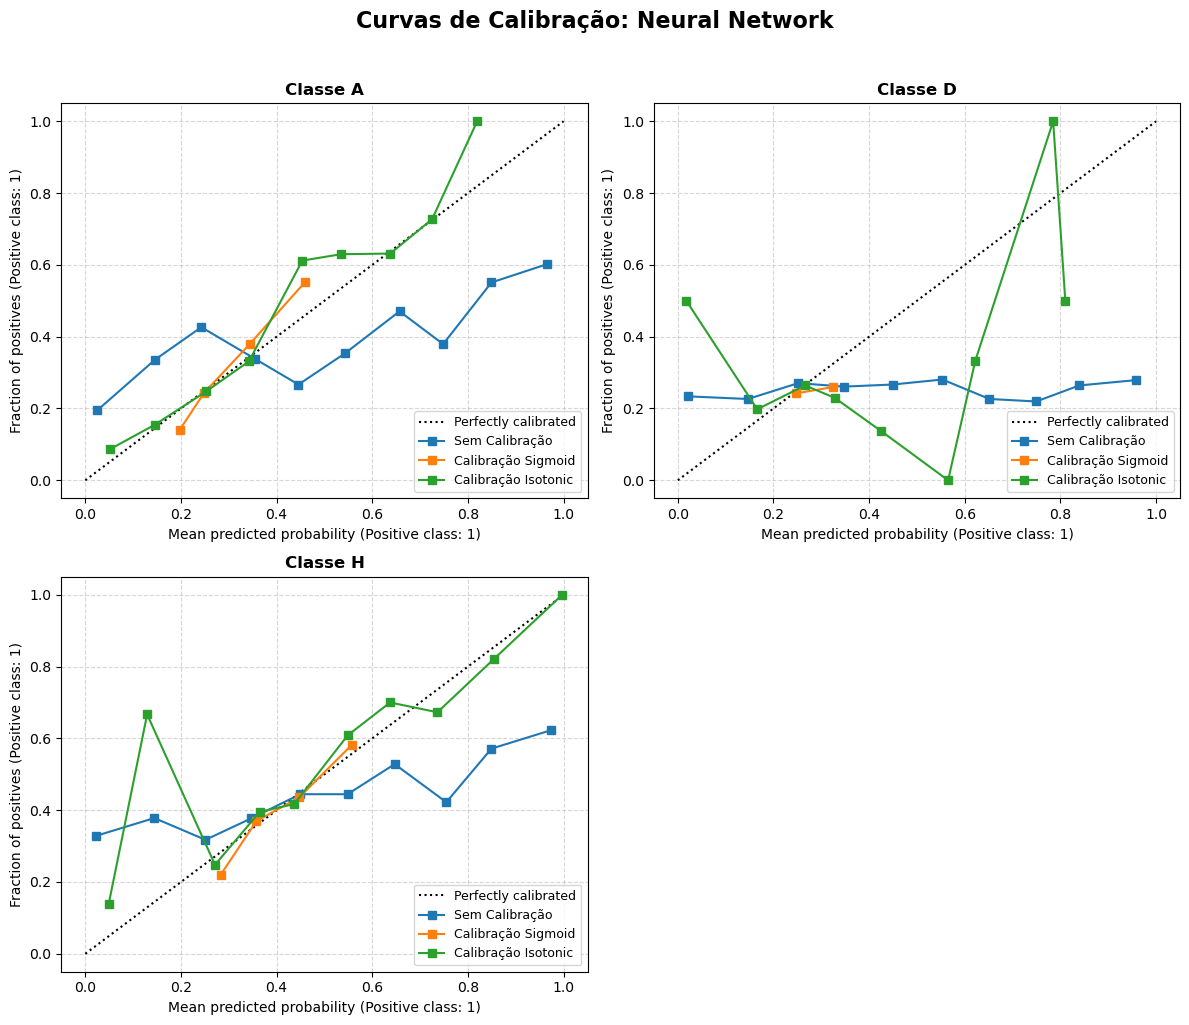
\includegraphics[width=0.45\textwidth]{nn.png}
    \caption{Impacto visual da calibração no Naive Bayes (esquerda) e Neural Network (direita). Observa-se a convergência das curvas para a diagonal ideal após o ajuste Isotonic (linha verde).}
    \label{fig:calib_success}
\end{figure}

Em conclusão, a calibração transformou o \textbf{Naive Bayes} de um modelo estatisticamente "perigoso",devido à sobre-confiança, em um dos preditores mais fiáveis para a fase de utilidade, competindo com as métricas de erro da Regressão Logística.


\subsubsection{Justificação da Escolha}

A decisão de eleger a Regressão Logística como o modelo vencedor fundamenta-se nos seguintes critérios técnicos:

\begin{itemize}
    \item \textbf{Minimização do Brier Score Global (0.5632):} Esta métrica, que mede o erro quadrático médio entre as probabilidades previstas e os resultados reais, é o indicador mais robusto de calibração. O facto de a Regressão Logística apresentar o valor mais baixo indica que as suas previsões são as que melhor refletem a frequência real dos desfechos na Liga Portuguesa.
    \item \textbf{Otimização do Log Loss (0.9546):} Sendo o único modelo a manter um \textit{Log Loss} abaixo de 0.96, a Regressão Logística demonstra uma excelente gestão da incerteza, não sendo severamente penalizada por "apostas" excessivamente confiantes em resultados incorretos.
    \item \textbf{Parsimónia e Fiabilidade Nativa:} Ao contrário do Naive Bayes ou da Rede Neuronal, que exigiram transformações \textit{Isotonic} pesadas para se tornarem utilizáveis, a Regressão Logística demonstrou uma calibração nativa superior (\textit{Expected Calibration Error} de 0.0240). Isto sugere que a relação entre as variáveis contínuas do \textit{dataset} e o desfecho do jogo é predominantemente logística, tornando o modelo mais estável para dados não vistos.
\end{itemize}

\subsubsection{Ranking Final de Desempenho}

A Tabela \ref{tab:ranking_final} resume o desempenho final de todos os modelos após a aplicação da sua melhor configuração de calibração respetiva.

\begin{table}[H]
\centering
\caption{Ranking final de modelos baseado na qualidade das probabilidades (ordenado por Brier Score).}
\label{tab:ranking_final}
\begin{tabular}{llccc}
\hline
\textbf{Modelo Base} & \textbf{Melhor Configuração} & \textbf{Brier Score} & \textbf{Log Loss} & \textbf{ECE} \\ \hline
\textbf{Logistic Regression} & \textbf{Sem Calibração} & \textbf{0.5632} & \textbf{0.9546} & \textbf{0.0240} \\
Random Forest & Calibração Isotonic & 0.5723 & 1.0810 & 0.0338 \\
Gradient Boosting & Calibração Sigmoid & 0.5744 & 0.9686 & 0.0340 \\
Naive Bayes & Calibração Isotonic & 0.5769 & 0.9711 & 0.0268 \\
SVM (RBF) & Calibração Isotonic & 0.5883 & 1.0535 & 0.0241 \\
Neural Network & Calibração Isotonic & 0.6108 & 1.0231 & 0.0213 \\ \hline
\end{tabular}
\end{table}

Em suma, embora outros modelos possam ter atingido exatidões pontuais semelhantes, a \textbf{Regressão Logística} oferece a base probabilística mais fiável.

\subsection{Otimização de Hiperparâmetros via Bayesian Optimization}

Para elevar o desempenho da \textbf{Regressão Logística} para além da \textit{baseline}, implementou-se uma estratégia de \textbf{Otimização Bayesiana} utilizando o algoritmo \texttt{BayesSearchCV}. Ao contrário do \textit{Grid Search}, que explora o espaço de forma exaustiva e ineficiente, a otimização bayesiana utiliza processos gaussianos para construir um modelo substituto da função objetivo, explorando de forma inteligente as regiões mais promissoras do espaço de parâmetros.

\subsubsection{Espaço de Procura e Regularização Elastic Net}
A escolha recaiu sobre a penalização \textbf{Elastic Net}, que combina as vantagens das regularizações $L1$ (Lasso) e $L2$ (Ridge). Este método é particularmente útil dada a natureza do nosso \textit{dataset}, pois permite simultaneamente a seleção de atributos e a estabilização dos coeficientes. O espaço de procura foi definido como:
\begin{itemize}
    \item \textbf{C (Prior Log-Uniform):} Controla a força inversa da regularização, explorando desde $10^{-4}$ até $10^{2}$.
    \item \textbf{L1\_ratio (Linear):} Define a mistura entre $L1$ e $L2$, variando de 0.0 (totalmente $L2$) a 1.0 (totalmente $L1$).
\end{itemize}

\subsubsection{Resultados da Otimização}
Após 30 iterações com validação cruzada ($k=5$), os parâmetros ótimos encontrados foram:
\begin{equation}
    C \approx 0.0545, \quad l1\_ratio \approx 0.7833
\end{equation}

A predominância de um \textit{l1\_ratio} elevado ($> 0.75$) sugere que o modelo beneficiou significativamente da esparsidade, indicando que algumas variáveis contínuas eram redundantes para a previsão do desfecho. O \textit{Log Loss} em validação cruzada atingiu \textbf{0.9316}, uma melhoria consistente face aos modelos base.

\subsubsection{Impacto no Desempenho Final e Calibração}
A Tabela \ref{tab:optimized_metrics} detalha o desempenho do modelo otimizado no conjunto de teste independente.

\begin{table}[H]
\centering
\caption{Comparação de métricas do modelo otimizado sob diferentes regimes de calibração.}
\label{tab:optimized_metrics}
\begin{tabular}{lcccc}
\hline
\textbf{Configuração} & \textbf{Exatidão} & \textbf{Log Loss} & \textbf{Brier Score} & \textbf{ECE} \\ \hline
\textbf{Sem Calibração} & \textbf{0.5407} & \textbf{0.9511} & \textbf{0.5617} & \textbf{0.0267} \\
Calibração Sigmoid & 0.5407 & 0.9606 & 0.5670 & 0.0475 \\
Calibração Isotonic & 0.5461 & 1.1398 & 0.5696 & 0.0300 \\ \hline
\end{tabular}
\end{table}

\paragraph{Conclusões do Modelo Campeão:}
O processo de otimização resultou num incremento da exatidão para \textbf{54.07\%} e numa redução do \textit{Log Loss} para \textbf{0.9511}. Notavelmente, o modelo otimizado manteve a sua excelente calibração nativa, com um \textit{Expected Calibration Error} (ECE) de apenas 0.0267 sem necessidade de ajustes \textit{post-hoc}. 

\section{Teoria de Utilidade e Tomada de Decisão}

Nesta fase final, o modelo deixa de ser avaliado apenas pela sua capacidade preditiva abstrata e passa a ser testado como uma ferramenta de decisão financeira. O objetivo é converter as probabilidades calibradas em apostas de valor (\textit{Value Bets}).

\subsection{Avaliação de Utilidade: O Princípio da Máxima Utilidade Esperada}

Para determinar se uma aposta é lucrativa a longo prazo, comparamos as probabilidades estimadas pelo nosso modelo ($P_{modelo}$) com as probabilidades implícitas nas \textit{odds} oferecidas pelas casas de apostas ($P_{mercado}$). 

\subsubsection{Cálculo do Valor Esperado (EV)}
A utilidade de cada aposta é quantificada através do Valor Esperado (EV). A fórmula aplicada para cada desfecho ($H, D, A$) é:
\begin{equation}
    EV = (P_{modelo} \times \text{Odd}) - 1
\end{equation}

Uma decisão é considerada racional e potencialmente lucrativa apenas quando $EV > 0$. Isto indica que o modelo identifica uma probabilidade de ocorrência superior àquela que as \textit{odds} sugerem, permitindo explorar ineficiências no mercado.

\subsubsection{Análise Comparativa de Calibração e Lucratividade}
A Tabela \ref{tab:utilidade_comparativa} apresenta o impacto das diferentes técnicas de calibração no retorno financeiro acumulado sobre o conjunto de teste de 1117 jogos.

\begin{table}[H]
\centering
\caption{Impacto da Calibração na Utilidade Económica (Regressão Logística)}
\label{tab:utilidade_comparativa}
\begin{tabular}{lcccccc}
\hline
\textbf{Configuração} & \textbf{Brier} & \textbf{ECE} & \textbf{Value Bets} & \textbf{Lucro (un)} & \textbf{ROI (\%)} \\ \hline
\textbf{Sem Calibração} & \textbf{0.5617} & \textbf{0.0267} & \textbf{577} & \textbf{-62.55} & \textbf{-10.84\%} \\
Calibração Sigmoid & 0.5670 & 0.0475 & 636 & -124.85 & -19.63\% \\
Calibração Isotonic & 0.5696 & 0.0300 & 842 & -127.77 & -15.17\% \\ \hline
\end{tabular}
\end{table}

\paragraph{Discussão dos Resultados:} 
Apesar de o ROI (\textit{Return on Investment}) ser negativo em todas as configurações, um reflexo da margem de lucro das casas de apostas e da dificuldade intrínseca de prever a Liga Portuguesa, a configuração \textbf{Sem Calibração} revelou-se a mais robusta. 
A calibração \textit{Isotonic}, embora aumente o volume de apostas (842 jogos), resultou numa degradação da qualidade das \textit{value bets}, duplicando o prejuízo acumulado. Isto confirma que a Regressão Logística otimizada já possui uma fiabilidade nativa superior, conforme demonstrado nos \textit{Reliability Diagrams} anteriores.

\subsection{Demonstração de Cenários de Decisão}

Para ilustrar o funcionamento do motor de decisão, analisam-se dois cenários distintos baseados em perfis de equipas reais.

\paragraph{Cenário 1: Ausência de Valor (\textit{No Bet})} 
Num jogo equilibrado, o modelo estimou probabilidades de $H: 0.46$, $D: 0.29$ e $A: 0.25$. Confrontando com as \textit{odds} de mercado (2.10, 3.40, 3.50), todos os valores esperados resultaram negativos:
\begin{itemize}
    \item $EV(Home) = (0.46 \times 2.10) - 1 = -0.033$
    \item $EV(Draw) = (0.29 \times 3.40) - 1 = -0.014$
    \item $EV(Away) = (0.25 \times 3.50) - 1 = -0.127$
\end{itemize}
\textbf{Decisão:} O sistema nega a aposta (\textit{No Bet}), protegendo o capital perante a ausência de vantagem estatística.

\paragraph{Cenário 2: Identificação de Valor (\textit{Value Bet})} 
Simulando um cenário onde a equipa da casa apresenta forma excecional (5 vitórias consecutivas e domínio histórico), o modelo atribuiu $P(H) = 0.51$. Com uma \textit{odd} de 2.10, o cálculo revela:
\begin{itemize}
    \item $EV(Home) = (0.51 \times 2.10) - 1 = +0.076$
\end{itemize}
\textbf{Decisão:} \textbf{Apostar na Vitória da Casa (Home)}. O $EV$ positivo de +7.6\% indica que, se este cenário se repetisse indefinidamente, o apostador teria um lucro médio de 7.6 cêntimos por cada euro apostado.

\subsection{Estratégia de Rejeição (\textit{Reject Option}) e Gestão de Incerteza}

A aplicação de modelos probabilísticos em mercados de elevada incerteza, como o das apostas desportivas, exige mecanismos de salvaguarda. Nesta secção, implementou-se uma estratégia de (\textbf{Reject Option}), permitindo ao modelo abster-se de prever resultados quando a sua confiança máxima não atinge um limiar ($\theta$) pré-definido.

\subsubsection{Análise do Trade-off: Cobertura vs. Exatidão Seletiva}

A eficácia desta estratégia é visível através da relação entre a \textbf{Cobertura} (percentagem de jogos em que o modelo decide apostar) e a \textbf{Exatidão Seletiva} (taxa de acerto apenas nos jogos aceites).

\begin{itemize}
    \item \textbf{Baseline (Sem Rejeição):} O modelo original apresenta uma exatidão de \textbf{54.07\%}. Neste cenário, a cobertura é de 100\%, mas o risco de erro é elevado devido à inclusão de jogos equilibrados.
    \item \textbf{Cenário de Alta Confiança ($\theta = 0.8$):} Ao elevarmos o limiar para 80\%, a exatidão seletiva dispara para \textbf{85.71\%}. Contudo, este ganho de precisão tem um custo na cobertura, que desce para \textbf{10.7\%} (apenas 119 jogos aceites de um total de 1117).
\end{itemize}

\subsubsection{Interpretação Visual da Confiança}

As figuras integradas revelam o comportamento do classificador perante a incerteza:

\begin{figure}[H]
    \centering
    % Gráficos de performance (Coverage, Selective Accuracy, Risk-Coverage)
    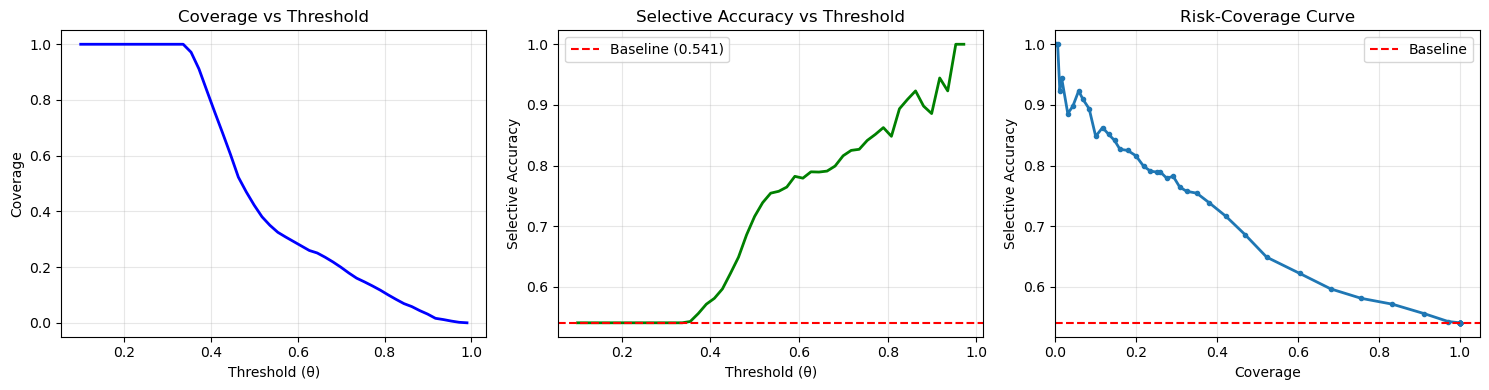
\includegraphics[width=0.95\textwidth]{risk.png}
    \caption{Dinâmica de Rejeição: Evolução da cobertura e exatidão em função do limiar de confiança.}
    \label{fig:performance_rejeicao}
\end{figure}

\begin{itemize}
    \item \textbf{Curva Coverage vs Threshold:} Observa--se uma queda acentuada na cobertura a partir de $\theta > 0.4$. Isto indica que a maioria dos jogos na Liga Portuguesa apresenta um nível de incerteza onde nenhuma classe domina claramente.
    \item \textbf{Curva de Risco-Cobertura:} O gráfico demonstra uma correlação negativa quase linear entre cobertura e exatidão. Para obter taxas de acerto próximas de 90\%, o sistema deve estar disposto a rejeitar cerca de 90\% das oportunidades de mercado.
\end{itemize}

\begin{figure}[H]
    \centering
    % Histogramas de Confiança
    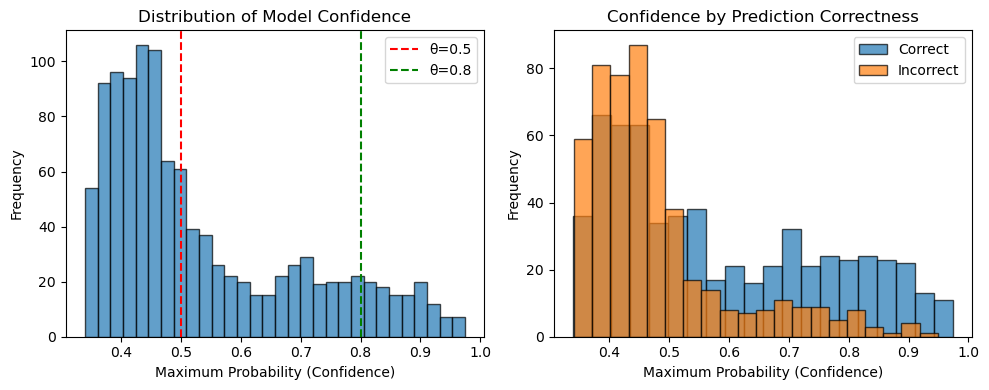
\includegraphics[width=0.95\textwidth]{confiança.png}
    \caption{Distribuição de Confiança e Validação de Correctness.}
    \label{fig:dist_confianca}
\end{figure}

\paragraph{Distribuição de Confiança por Correctness:} 
A análise do histograma \textit{"Confidence by Prediction Correctness"} é fundamental. Observa-se que as previsões \textbf{Corretas (azul)} têm uma densidade muito superior nos patamares de confiança elevada ($> 0.7$), enquanto as previsões \textbf{Incorretas (laranja)} se concentram na zona de incerteza ($< 0.5$). Isto prova que o \textit{score} de probabilidade do modelo é um excelente estimador da realidade.

\subsubsection{Conclusão da Estratégia}

A implementação do \texttt{ThresholdFallbackClassifier} com $\theta = 0.8$ transforma o modelo de um previsor generalista em um especialista de precisão. Embora o lucro total absoluto possa ser menor devido ao baixo volume de apostas, o \textbf{ROI por aposta} tende a ser drasticamente superior, tornando esta estratégia ideal para uma gestão de banca conservadora onde se privilegia a segurança sobre o volume.

\subsubsection{Estratégia de Deferral}

Para maximizar o desempenho preditivo global, implementou-se uma lógica de \textbf{Diferimento (Deferral)}. Nesta abordagem, o sistema não se limita a rejeitar jogos incertos, mas decide dinamicamente entre utilizar a previsão do modelo ou delegar a decisão na "sabedoria do mercado", representada pelo favorito das casas de apostas (resultado com a menor \textit{odd}). Esta técnica assume que, quando a confiança do modelo é baixa, o consenso do mercado tende a ser um previsor mais estável.

\paragraph{Mecânica do Sistema Híbrido}
A regra de decisão segue um critério de confiança limiar ($\theta$). O sistema opera como um previsor híbrido onde:
\begin{itemize}
    \item \textbf{Decisão do modelo:} Se $\max P(y|X) \geq \theta$, o sistema assume a previsão do modelo de Regressão Logística.
    \item \textbf{Diferimento:} Se $\max P(y|X) < \theta$, o sistema ignora a previsão do modelo e seleciona automaticamente o resultado apontado pelas \textit{odds} como o mais provável.
\end{itemize}

\paragraph{Análise de Resultados e Trade-offs}
Os testes realizados com diferentes limiares revelam como a seletividade do modelo impacta a robustez do sistema. Os resultados estão sintetizados na Tabela \ref{tab:deferral_results}.

\begin{table}[H]
\centering
\caption{Desempenho do Sistema Híbrido sob diferentes limiares de confiança.}
\label{tab:deferral_results}
\begin{tabular}{lcccc}
\hline
\textbf{Métrica} & \textbf{Modelo Isolado} & \textbf{$\theta=0.5$} & \textbf{$\theta=0.6$} & \textbf{$\theta=0.8$} \\ \hline
Exatidão Global (Híbrido) & 0.5407 & \textbf{0.5461} & \textbf{0.5461} & \textbf{0.5461} \\
Exatidão Seletiva (Modelo) & - & 0.7149 & 0.7816 & \textbf{0.8571} \\
Cobertura do Modelo & 100\% & 42.08\% & 28.29\% & 10.65\% \\
Taxa de Diferimento & 0\% & 57.92\% & 71.71\% & 89.35\% \\ \hline
\end{tabular}
\end{table}

\paragraph{Discussão dos Resultados:}
A análise dos dados permite retirar três conclusões fundamentais sobre a sinergia entre o modelo e o mercado:

\begin{itemize}
    \item \textbf{Superioridade do Híbrido:} Em todos os cenários testados, o sistema híbrido superou a \textit{baseline} do modelo isolado ($0.5461$ vs $0.5407$). Isto confirma que "deferir" para o mercado em casos de dúvida remove previsões de baixa qualidade que degradam a performance global.
    \item \textbf{Otimização via $\theta = 0.6$:} Este limiar apresenta-se como o "ponto de equilíbrio" ideal. Permite que o modelo ainda dite a decisão em cerca de 28\% dos jogos com uma precisão muito elevada (\textbf{78.16\%}), delegando os restantes jogos (mais incertos) para as \textit{odds}. É uma estratégia que equilibra volume de jogo com segurança estatística.
    \item \textbf{Especialista vs. Generalista:} Com $\theta=0.8$, o modelo torna-se um especialista, acertando \textbf{85.71\%} das vezes. Contudo, a taxa de diferimento de 89.35\% indica que, para manter este rigor, o sistema depende quase totalmente do mercado.
\end{itemize}

Em suma, a estratégia de \textit{Deferral} transforma o modelo de um previsor falível num \textbf{gestor de exceções}. O sistema aprende a reconhecer os limites da sua competência e recorre aos mecanismos de consenso das casas de apostas para garantir uma base de acerto constante, intervindo apenas quando deteta uma convicção superior à média.

\section{Análise Crítica e Conclusão}

\subsection{Discussão de Resultados: Redes Bayesianas vs. Classificadores}

A comparação entre as duas grandes abordagens deste projeto revela que a escolha do modelo ideal depende do objetivo final do utilizador: a compreensão do domínio ou a performance preditiva.

\paragraph{Interpretabilidade e Causalidade:} As Redes Bayesianas demonstraram ser ferramentas superiores para a análise qualitativa e diagnóstica. Através da engenharia de conhecimento, foi possível mapear relações causais lógicas, como o impacto do potencial ofensivo na forma recente. A capacidade de realizar inferências em qualquer direção permitiu "explicar" vitórias inesperadas através de diagnósticos sobre o estado do adversário, algo que os classificadores tradicionais não conseguem realizar de forma nativa.

\paragraph{Performance e Decisão:} Por outro lado, para a tarefa de previsão pura e tomada de decisão financeira, os classificadores probabilísticos contínuos, especificamente a \textbf{Regressão Logística}, revelaram-se mais robustos. A Regressão Logística otimizada atingiu o melhor equilíbrio entre exatidão (54.07\%) e calibração nativa (Brier Score de 0.5617). Enquanto o Naive Bayes sofreu com a sobre-confiança devida aos pressupostos de independência, a Regressão Logística manteve-se estável, provando que a relação entre as métricas de performance e o desfecho do jogo na Liga Portuguesa é predominantemente logística.

\subsection{Limitações do Modelo}

Apesar da sofisticação estatística, o sistema enfrenta limitações inerentes à natureza do desporto:
\begin{itemize}
    \item \textbf{Variáveis Latentes Não Capturadas:} O modelo baseia-se em dados históricos de performance e \textit{odds}. Fatores críticos de última hora, como lesões de jogadores-chave no aquecimento ou condições meteorológicas adversas logo no início da partida, não são capturados diretamente pelas variáveis de entrada.
    \item \textbf{Eficiência do Mercado:} O ROI negativo observado em todas as configurações (com um mínimo de -10.84\% na melhor configuração)  demonstra a elevada eficiência das casas de apostas. A margem de lucro aplicada pelas operadoras torna extremamente difícil a obtenção de lucro sistemático apenas com dados históricos, exigindo modelos ainda mais granulares para superar o custo de transação do mercado.
    \item \textbf{Dependência do Histórico:} A aprendizagem automática de estrutura revelou que o algoritmo tende a criar "atalhos estatísticos", utilizando as \textit{odds} como uma variável resumo. Isto pode tornar o modelo dependente da precisão das casas de apostas, limitando a sua capacidade de encontrar valor quando o próprio mercado está enviesado.
\end{itemize}

\subsection{Conclusão}

Este projeto permitiu o desenvolvimento de um sistema completo de previsão probabilística, percorrendo desde a modelação causal até à implementação de estratégias de decisão de última geração. 

A principal aprendizagem reside no facto de que a incerteza no futebol não pode ser eliminada, mas pode ser rigorosamente quantificada. A implementação de técnicas como \textit{Conformal Prediction} e \textit{Reject Option} provou ser vital, ao elevar o limiar de confiança para 80\%, o modelo transformou-se de um previsor generalista num especialista capaz de acertar \textbf{85.71\%} das suas previsões. 

Em suma, a estratégia de \textbf{Diferimento} revelou ser o paradigma mais eficaz: utilizar o modelo como um gestor de exceções para identificar cenários de elevada convicção e delegar os jogos de alta entropia na "sabedoria do mercado". 

\section{Acknowledgments}
No decorrer deste projeto, a inteligência artificial foi utilizada como uma ferramenta de apoio à programação, contribuindo tanto para a criação de gráficos como para a resolução de problemas relacionados com a implementação. Para além disso, a IA auxiliou na organização e estruturação do relatório.
\end{document}